\documentclass[
  a4paper,            % DIN A4
  DIV=10,             % Schriftgröße und Satzspiegel
  oneside,            % einseitiger Druck
  BCOR=5mm,           % Bindungskorrektur
  parskip=half,       % Halber Abstand zwischen Absätzen
  numbers=noenddot,   % Kein Punkt hinter Kapitelnummern
  bibtotoc,           % Literaturverzeichnis im Inhaltsverzeichnis
  listof=totoc        % Abbildungs- und Tabellenverzeichnis im Inhaltsverzeichnis
]{scrreprt}
\usepackage{style/thesisstyle}

\makeglossaries           % create all glossary entries (remember: run makeglossaries manually)
\loadglsentries{thesisglossaries.tex}  % load acronym, symbol and glossary entries

\sisetup{locale = UK}     % siunitx locale setup
%\DeclareSIUnit \fps{fps}  % a custom unit (usage: \SI{24}{\fps})

\begin{document}
% !TEX root = ../thesis.tex
%
% configurations
%

% English Language support
% -> uncomment if needed
% Beta!
\fullenglish{yes}
%\fullenglish{no}

% text field
%-> replace supervisor names with correct ones
\firstSupervisor{Prof. Dr. Thomas Schmidt}
\secondSupervisor{Prof. Dr. Franz Korf}

% text field
%-> replace title with your thesis title
\thesisTitle{Laufzeitkonfiguration von eingeschränkten Geräten über ein gemeinsames Betriebssystemmodul}
\thesisTitleEN{Runtime configuration of constrained devices via a shared operating system module}

% text field
%-> replace the key words with your own key words
\keywordsDE{Laufzeitkonfiguration, Eingebettete Geräte, IoT, Betriebssystem}
\keywordsEN{Runtime Configuration, Constrained Devices, IoT, Operating System}

% text field
%-> replace the text with a description of the thesis
\abstractDE{
    Viele Anwendungen im Internet der Dinge (IoT) verwenden Parameter, die zur Laufzeit geändert werden müssen.
    Typische Beispiele können Authentifizierungsdaten, die Abtastrate einer Messung oder eine LED-Farbe sein.
    Darüber hinaus sind in modernen Industrieumgebungen Laufzeitparameter von Geräten über Plug-and-Play-fähige Protokolle wie \gls{gl:lwm2m} usw. fernveränderbar.

    Gegenwärtig stellt \gls{gl:riot_os} keine \acrshort{ac:api} für Laufzeitparameter bereit.
    Stattdessen muss jede Anwendung benutzerdefinierte, oft redundante Logik für ihren spezifischen Anwendungsfall implementieren.
    Eine voll funktionsfähige Integration externer Konfigurationsmanager wie \gls{gl:lwm2m} erweist sich angesichts der enormen Menge an Treibern und Geräten, die für jedes einzelne Verwaltungstool unterstützt und gewartet werden müssen, als besonders schwierig.

    In dieser Arbeit wird eine Konfigurationsregistrierung auf Systemebene eingeführt, mit der man Parameterwerte zur Laufzeit setzen und abzurufen kann.
    Sie organisiert die Parameter nach einem standardisierten Schema, das Typinformationen und andere Metadaten wie Name und Beschreibungsfelder enthält, um sie anderen Modulen wie Konfigurationsmanagern zugänglich zu machen.
    Die Parameterwerte werden optional im lokalen Speicher gehalten.
    Um die Parameter zu ändern, werden eine CLI und Schnittstellen zu \acrshort{ac:coap}, \gls{gl:mqtt} und \gls{gl:lwm2m} spezifiziert.
    Darüber hinaus werden in dieser Arbeit wichtige Entscheidungen zum \acrshort{ac:api}-Design diskutiert und erläutert, warum standardisierte, modulunabhängige Schemata für gemeinsame Konfigurationsparameter für die Integration von externen Management-Tools wie \gls{gl:lwm2m} notwendig sind.
}
\abstractEN{
    Many applications on the Internet of Things (IoT) use parameters that need to be changed at runtime.
    Typical examples can be authentication credentials, the sampling rate of a measurement or an LED color.
    Furthermore in modern industrial spaces runtime parameters of devices are remotely changeable using plug-and-play capable protocols such as \gls{gl:lwm2m} etc.

    As of today, \gls{gl:riot_os} does not provide an \acrshort{ac:api} for runtime parameters.
    Instead, each application needs to implement custom, often redundant logic for its specific use case.
    A fully featured integration of external \glspl{gl:configuration_manager} such as \gls{gl:lwm2m} proves to be particularly difficult given the vast amount of drivers and devices that need to be supported and maintained for every single management tool.

    In this thesis we introduce a system-level configuration registry that allows for setting and getting configuration parameter values at runtime.
    It organizes parameters according to a standardized schema that includes type information and other metadata such as name and description fields to make them accessible to other modules such as \glspl{gl:configuration_manager}.
    The parameter values are optionally persisted on local storage.
    To change the parameters we specify a CLI and interfaces to \acrshort{ac:coap}, \gls{gl:mqtt} and \gls{gl:lwm2m}.
    Furthermore, we discuss important \acrshort{ac:api} design decisions and explain why standardized, module-independent schemas for common configuration parameters are essential for the integration of external management tools such as \gls{gl:lwm2m}.
}

% text field
%-> replace john with your name
\thesisAuthor{Lasse Jonas Rosenow}

% text field
%-> enter the submission date
\submissionDate{February 1, 2023}

% switch - uncomment only one
%-> uncomment NDA or public
%\NDA{yes}
\NDA{no}

% switch - uncomment only one
%-> uncomment old standard cover or cover Corporate Design 2017
\Cover{CD2017}
%\Cover{CD2017NoLogo}
%\Cover{Std2018}
%\Cover{Std2018_green} 			% with green bar

% switch - uncomment only one
%-> uncomment to show list of figures or not
\ListOfFigures{yes}
%\ListOfFigures{no}

% switch - uncomment only one
%-> uncomment to show list of tables or not
\ListOfTables{yes}
%\ListOfTables{no}

% switch - uncomment only one
%-> uncomment to show list of listings or not
\ListOfListings{yes}
%\ListOfListings{no}

% switch - uncomment only one
%-> uncomment to show list of acronyms or not
\ListOfAccronyms{yes}
%\ListOfAccronyms{no}

% switch - uncomment only one
%-> uncomment to show list of symbols or not
\ListOfSymbols{yes}
%\ListOfSymbols{no}

% switch - uncomment only one
%-> uncomment to show list of glossary entries or not
\Glossary{yes}
%\Glossary{no}

% switch - uncomment only one
%-> uncomment the study course you are in
\studycourse{ITS}
%\studycourse{TI}
%\studycourse{AI}
%\studycourse{WI}
%\studycourse{EI}
%\studycourse{REE}
%\studycourse{BMP}		
%\studycourse{BMP-hp}	 % Internship Report in M&P
%\studycourse{BMT}
%\studycourse{BMT-st}    % Study / home assignment in BMT
%\studycourse{BMT-hp}    % Internship Report in BMT
%\studycourse{MI}
%\studycourse{MIK}
%\studycourse{MA}
    % load all settings

\hyphenation{Ba-che-lor-the-sis Mas-ter-the-sis}

% Cover page here, no page number
\ICoverPage

% PDF Metadata
% !TEX root = ../thesis.tex
%
% PDF Metadata integration
% @author Thomas Lehmann
%

% PDF Metadata
\hypersetup{
pdftitle={\IthesisTitleEN},
pdfauthor={\IthesisAuthor},
pdfkeywords={\IkeyWordsEN}
}

% Titlepage is page one even if the number is not shown.
\pagenumbering{roman}
% Title page here
% !TEX root = ../thesis.tex
%
% title page
% @author Thomas Lehmann
% Hints for title page and page numbering: https://en.wikipedia.org/wiki/Title_page
%
\title{\IthesisTitle}   % set latex default title to be used by hyperref in pdf
\author{\IthesisAuthor} % set latex default author to be used by hyperref in pdf

\newpage
\thispagestyle{empty}
{\fontfamily{phv}\selectfont
  \hfuzz=20pt       % suppress warnings due to extension onto page margins

  % Author of thesis
  \vspace*{1cm}
  \begin{minipage}[b]{\textwidth}
    \fontsize{14pt}{20pt}
    \selectfont
    \begin{center}
      \IthesisAuthor
    \end{center}
  \end{minipage}

  % Title of thesis
  \vspace{1.5cm}
  \begin{minipage}[b][0cm][t]{\textwidth}
    \fontsize{18pt}{20pt}
    \selectfont
    \begin{center}
      \IthesisTitleEN
    \end{center}
  \end{minipage}

  % Important information
  \begin{textblock*}{\textwidth}(40mm,210mm)
    \begin{minipage}[b]{\textwidth}
      \hbadness=10001    % suppress underfull warning due to short text
      \fontfamily{cmr}\selectfont
      \fontsize{12pt}{14pt}
      \selectfont
      \ifdefined\ILanguageEN
        \IthesisKindEN ~submitted for examination in \IthesisExaminationEN \\
        in the study course \textit{\IstudyCourseName} \\
        at the \IthesisDepartmentFullEN \\
        at the \IthesisFacultyFullEN \\
        at University of Applied Science Hamburg\\

        Supervisor: \IfirstSv \\
        \ifdefined\IisTermPaper
          % left blank
        \else
          \ifdefined\IisInternshipReport
	  Supervised: \IsecondSv\\
          \else
        Supervisor: \IsecondSv \\
          \fi\fi
        
        Submitted on: \ISubDate \\
      \else
      	\ifdefined\IisInternshipReport
        \IthesisKindDE ~eingereicht im Rahmen des \IthesisExaminationDE \\	
	\else
        \IthesisKindDE ~eingereicht im Rahmen der \IthesisExaminationDE \\
        \fi
	im Studiengang \textit{\IstudyCourseName} \\
        am \IthesisDepartmentFull \\
        der \IthesisFacultyFull \\
        der Hochschule für Angewandte Wissenschaften Hamburg\\

        Betreuender Prüfer: \IfirstSv \\
        \ifdefined\IisTermPaper
          % left blank
        \else
          \ifdefined\IisInternshipReport
        betriebliche Betreuung: \IsecondSv \\							
	  \else
        Zweitgutachter: \IsecondSv \\
        \fi\fi

        Eingereicht am: \ISubDate \\
      \fi
    \end{minipage}
  \end{textblock*}
}


% Abstract page here
% !TEX root = ../thesis.tex
%
% abstract page
% @author Thomas Lehmann
%
\newpage
\thispagestyle{plain}
\clearpage
\hfuzz=12pt       % suppress warnings due to extension onto page margins


\textbf{\IthesisAuthor}

\vspace{0.3cm}
\textbf{Title of thesis}

\IthesisTitleEN

\vspace{0.3cm}
\textbf{Keywords}

\begin{minipage}{\textwidth}
  \IkeyWordsEN
\end{minipage}

\vspace{0.3cm}
\textbf{Abstract}

\IabstractEN


\newpage
\thispagestyle{plain}
\clearpage


\textbf{\IthesisAuthor}

\vspace{0.3cm}
\textbf{Thema der Arbeit}

\IthesisTitle

\vspace{0.3cm}
\textbf{Stichworte}

\IkeyWordsDE

\vspace{0.3cm}
\textbf{Kurzzusammenfassung}

\IabstractDE


% Table of contents here
\tableofcontents

% List of figures here
\IListOfFigures

% List of tables here
\IListOfTables

% List of listings here
\IListOfListings

% List of acronyms here
\IListOfAccronyms

% List of symbols here
\IListOfSymbols

% Uncomment if list of source code is needed (rarely).
%\lstlistoflistings  % requires package listings, needs to uncommenting of usepackage

% path to the folder is set to find the images used there
\graphicspath{ {assets/diagrams/}{assets/drawio/generated/} }

% Chapters
\clearpage
\pagenumbering{arabic}
\chapter{Introduction}
\label{chapter:introduction}

\section{Context}
\label{sec:introduction:context}

For constrained devices, it can be important not only to set certain configurations
before compiling and flashing a device but also while the device is in full operation, for example to change the rate or precision of a measurement or to update authentication credentials.
Also, it is often required to persist these values, so that a device would keep its configuration after a restart caused by a firmware update or power shortage for example.
It is also a common requirement to change these runtime configuration parameters via an external \gls{gl:configuration_manager} that communicates with the constrained device through \acrshort{ac:wlan}, Bluetooth, a serial bus, etc.
Not only smart home, but also more and more smart city applications require this external configuration management to be based on a standardized protocol such as \gls{gl:lwm2m} \cite{oma-lwm2m-core-12}, or the proprietary ``matter'' standard \cite{matter_standard} in smart home applications.
Using a standardized protocol gives the advantage of being able to automatically integrate a node into already existing systems without the need to write custom wrappers and also having the freedom to replace them with compatible devices implementing the same protocol.

\section{The Problem of Runtime Configuration in \gls*{gl:riot_os}}
\label{sec:introduction:problem}

As of today, there is no official way within \gls{gl:riot_os} \cite{bghkl-rosos-18} for modules to expose runtime configurable parameters, as can be seen in its official documentation \cite{riot_documentation}.
As a consequence, every application needs to implement its own way to work around this, causing a lot of duplicated work for all vendors using \gls{gl:riot_os} and also leading to large inconsistencies in their custom implementations making it impossible to easily integrate different devices.
For example, if there is a smart bulb vendor ``A'' and a smart bulb vendor ``B'', which both need to be controlled by a control unit made by vendor ``C'', this control unit would need to implement the custom \gls{ac:api} of vendor ``A'' and vendor ``B''.
Causing not only a huge amount of unnecessary work for vendor ``A'' and vendor ``B'' but also vendor ``C''.

\section{Thesis Aims and Objectives}
\label{sec:introduction:aims_and_objectives}

In this thesis we aim to investigate how to design an architecture that will extend the \gls{gl:riot_os} so that modules can expose configuration parameters in a way that they can easily integrate with external management tools such as \gls{gl:lwm2m}.
We also want to persist these values beyond device restarts.

\section{Thesis Structure}
\label{sec:introduction:structure}

In \autoref{chapter:background} we start by explaining the importance of configuration for constrained devices and the differences between static and runtime configuration.
Furthermore, we discuss why it is beneficial to implement this feature on an operating system level instead of per application.

In \autoref{chapter:requirements} we explain what kind of requirements the new \nameref{sec:design:riot_registry} is supposed to fulfill and discuss why these requirements are needed.

In \autoref{chapter:related_work} we first present existing academic work and discuss similarities and differences to our requirements.
Then we present existing implementation work and analyze in how much each of it fulfills the in \autoref{chapter:requirements} explained requirements.
After that, we conclude if one of the previously assessed work already fulfills enough requirements to just be implemented inside \gls{gl:riot_os} as its official \gls{ac:rcs}, or if the architecture for the \nameref{sec:design:riot_registry} will only be based on one of the previously analyzed work but extend its functionality, or if a completely new architecture needs to be designed and implemented.

In \autoref{chapter:design} we present the design of the \nameref{sec:design:riot_registry} that fulfills all the requirements from \autoref{chapter:requirements}.
We explain all the behavioral aspects, \gls{ac:api} decisions, and how the specific requirements from \autoref{chapter:requirements} are fulfilled.

In \autoref{chapter:implementation} we explain the implementation of the in \autoref{chapter:design} presented architecture, going more into detail as to how and why the more technical decisions of the \gls{ac:api} design were made.

In \autoref{chapter:testing} we explain how the correctness of the main \gls{ac:api} functions of the in \autoref{chapter:implementation} implemented source code is tested.

In \autoref{chapter:evaluation} we evaluate the overhead of the \nameref{sec:design:riot_registry} implementation (see \autoref{chapter:implementation}).
First, we measure the stack consumption of the main \nameref{sec:design:riot_registry} functions, then we discuss the results of these measurements.
Second, we measure the ROM size of the \nameref{sec:design:riot_registry} implementation and also discuss our findings.

In \autoref{chapter:future_work} we explain which steps are next to continue on the work of this thesis and how to further iterate upon it.

In \autoref{chapter:conclusion} we conclude on how successful this work is in fulfilling its aims set in \autoref{sec:introduction:aims_and_objectives} and more specifically in \autoref{chapter:requirements} and reflect on what lessons we have learned in the process.

\chapter{Background of (OS) Configuration}
\label{chapter:background}

\section{The Importance of Configuration}
\label{sec:background:why_configuration_devices}

Configuration is a way of making a program flexible, so it can be used in scenarios that have different requirements and are not compatible with each other, without the need to maintain multiple versions of the program that are almost identical.
It i.e. allows hiding certain features behind a configuration flag or gives the possibility to change some internal values by exposing them via an external interface.

\section{Static vs. Dynamic Configuration}
\label{sec:background:static_vs_dynamic_configuration}

Most applications use static configuration parameters to become more flexible.
These static configuration parameters are set before the source code gets compiled to machine code and can not be changed after. They are constant values written to the program storage.
Typical use-cases are flags to enable/disable program features or parameters to configure which pins to use for i.e.\ I²C on a hardware board.
In the \gls{gl:riot_os}, this is typically done with the help of CFLAGS inside a Makefile \cite{gnu_make} or through Kconfig \cite{linux-kconfig-20} on more modern setups.
The benefit of static configuration is that in cases in which a dynamic configuration has no benefit, these configuration values are less simple to accidentally being mutated by some parts of the application as they can not be changed.
In general, every configuration parameter that does not need to be changed at runtime, as seen in the examples above, should be defined statically.

For some configuration parameters though it is necessary to be able to change them at runtime. These parameters must be dynamic and not static.
A common use-case is a ``smart'' RGB bulb. If its color value is static, it can only be changed by recompiling the program of the RGB bulb and flashing it to the RGB bulb flash storage.
But if it is dynamic, it can be changed at runtime, without the need to recompile the whole application.
To change runtime configuration parameters, they can be for example exposed through a \gls{ac:coap} \cite{RFC-7252} or \gls{gl:lwm2m} interface to enable external control.

Static and dynamic configurations can also be mixed by dynamically switching between a set of statically defined configurations.
For example, an application could run in ``IDLE'' or ``PERF'' mode.
Then it can be statically defined, what CPU frequency etc. must be used for ``IDLE'' or ``PERF''. It is possible to dynamically switch between these predefined modes \cite{4253243}.

\section{Benefits of an Operating System-Level Implementation}
\label{sec:background:benefits_of_an_operating_system_level_implementation}

Implementing a runtime configuration registry on an operating system level means that it can also benefit from the hardware abstractions provided by it.
For example, if the \nameref{sec:design:riot_registry} implements a \gls{ac:coap} \gls{ac:api} to enable external access to configuration values, this \gls{ac:coap} \gls{ac:api} relies on the \gls{gl:riot_os} network stack \cite{lkhpg-cwemr-18}. This network stack is then implemented by all the different target devices supported by \gls{gl:riot_os}.
This way the registry works on all the devices supported by \gls{gl:riot_os} and does not need to implement wrappers for every target device itself.

Besides the hardware abstraction, an operating system level implementation also comes with the benefit that it can integrate with all the modules/drivers that are already provided by the operating system itself \cite{riot_drivers}.
This way a \gls{gl:riot_os} application can just enable the registry feature and automatically get runtime configuration capabilities for all drivers or modules it depends on.
If the registry is written on an application level, it needs to implement the drivers/modules itself and then integrate them with the registry on a per-application basis, instead of writing it once for the operating system.
\chapter{Requirements of a Runtime Configuration System (RCS)}
\label{chapter:requirements}

To be able to assess how suitable existing related work is, or if it is necessary to design a completely new architecture to fulfill the requirements for runtime configuration inside \gls{gl:riot_os}, it is first necessary to define what is needed and why.

\section{Shared \acrlongpl*{ac:cs}}
\label{sec:requirements:shared_pre_defined_configuraiton_schemas}

A \glsfirst{ac:cs} is mostly a data structure combined with some additional metadata such as parameter types or preconditions.
For a \gls{gl:configuration_manager} to be easily integrated into other external tools, it is necessary to have a collection of \glspl{ac:cs} to describe common configuration needs.
For example, there could be an LED \gls{ac:cs} consisting of three unsigned 8-bit integer variables, or a WI-FI \gls{ac:cs} containing the SSID, the password, etc.
Now, these \glspl{ac:cs} are supposed to be implemented by for example LED drivers, or WI-FI module drivers.
This way the registry has a consistent \gls{ac:api}, as can be seen on the right-hand side of \autoref{fig:evaluation:requirements:shared_pre_defined_configuraiton_schemas}.

An alternative approach is to define a custom \gls{ac:cs} per module basis, as can be seen on the left-hand side of \autoref{fig:evaluation:requirements:shared_pre_defined_configuraiton_schemas}.
This results in a lot of duplicated work and inconsistent \glspl{ac:api} for equal operations.
The advantage of this approach is that the work put into defining the custom \gls{ac:cs} is less than specifying a \gls{ac:cs} that has to fit for all comparable use-cases.
So new modules/driver that require a certain configuration module that is for example not yet implemented in the registry would just specify their own and don't need to find a solution for all first.
This would save a lot of review time and helps adoption.

If each approach's advantages and disadvantages are compared, having a consistent \gls{ac:api} outweighs the time saving of a per-module approach and is worth spending some extra time for, as this extra work is not wasted, but essential to enable the integration of external \glspl{gl:configuration_manager}. With no consistent \gls{ac:api}, those tools would need to be adapted to every single driver instead of just the \glspl{ac:cs}, that are shared among modules.

\begin{figure}[H]
    \centering
    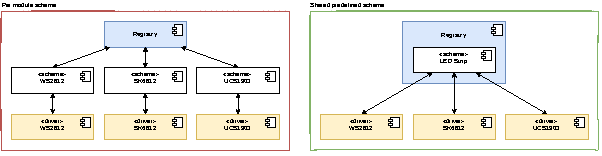
\includegraphics[width=\textwidth]{requirements_shared_pre_defined_configuration_schemas}
    \caption{Per module \glspl{ac:cs} (left-hand side) and Shared \glspl{ac:cs} (right-hand side).}
    \label{fig:evaluation:requirements:shared_pre_defined_configuraiton_schemas}
\end{figure}

\section{Multiple Instances per \acrlong*{ac:cs}}
\label{sec:requirements:multiple_instances_per_schema}

This requirement is strongly connected to \autoref{sec:requirements:shared_pre_defined_configuraiton_schemas}.
Having shared \glspl{ac:cs} requires that these can be used at the same time, by multiple modules, as can be seen on the right-hand side of \autoref{fig:evaluation:requirements:multiple_instances_per_schema}, without causing conflicts as can be seen on the left-hand side of \autoref{fig:evaluation:requirements:multiple_instances_per_schema}.
If an example application has 3 different LED modules, of which each implements the same LED \gls{ac:cs}, they need to expose their data in their instance of this \gls{ac:cs} and don't overwrite each other's configurations.
Besides that even if there is only one module, that is used to control three LEDs of the same kind, it is also necessary for this module to create multiple instances so that each LED can be configured on its own.

This means that the \gls{ac:cs} should not hold the actual data but only specify its structure.
Modules then shall be able to create as many instances of this \gls{ac:cs} as is needed.

\begin{figure}[H]
    \centering
    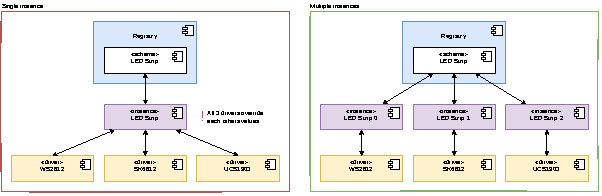
\includegraphics[width=\textwidth]{requirements_multiple_instances_per_schema}
    \caption{Single shared instance (left-hand side) and Multiple instances (right-hand side).}
    \label{fig:evaluation:requirements:multiple_instances_per_schema}
\end{figure}

\section{Integer Path as the Identifier of Configuration Values}
\label{sec:requirements:integer_path_as_identifier_of_configuration_values}

To uniquely identify each configuration parameter a path or array is needed that points to the parameter.
For example ``schema\_id/instance\_id/parameter\_id''.

One way to do this is using an array of strings, as can be seen on the left-hand side of \autoref{fig:evaluation:requirements:integer_path_as_identifier_of_configuration_values}, inspired by the URI in HTTP \cite{RFC-3986}.
This approach is very verbose, which is good for integrations such as \gls{gl:mqtt} \cite{mqtt311} or \gls{ac:coap}, which also rely on using string based identifier paths.
It is also significantly less difficult for humans to work with compared to numbers for example.
The downside of using strings is a huge amount of overhead, especially for constrained devices.
Not only in terms of processing power that is necessary to path strings compared to simple arrays of numbers, but most importantly in terms of unnecessary payload when accessed remotely.
For example through LoRA, which in some scenarios could make every single byte count \cite{avtms-ull-17}.

Using integers instead of strings does not come with these issues, but also has some disadvantages, such as a lower human readability, as can be seen on the right-hand side of \autoref{fig:evaluation:requirements:integer_path_as_identifier_of_configuration_values}.
But \gls{gl:riot_os} is an operating system for constrained devices and this is why low connectivity and low power scenarios are more important use-cases than human readability.
Also, if the parameter identifier is based on an integer path, it is possible to give parameters optional string identifiers to improve the integration of external tools and also improve human readability.
(Besides that modern IoT configuration protocols such as the \gls{ac:coap} Management Interface (CORECONF) \cite{draft-ietf-core-comi-11} also use integers as identifiers, which does not mean it is the right to choose in this case, but still strengthens the point.)

As a conclusion, integer arrays with optional string metadata fields are a solid solution for runtime configuration parameter identifiers of constrained devices.

\begin{figure}[H]
    \centering
    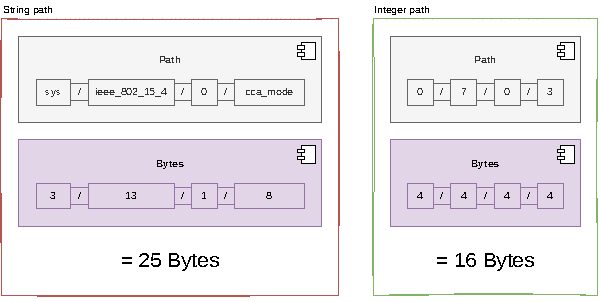
\includegraphics[width=\textwidth]{requirements_integer_path_as_identifier_of_configuration_values}
    \caption{String path (left-hand side) and Integer path (right-hand side).}
    \label{fig:evaluation:requirements:integer_path_as_identifier_of_configuration_values}
\end{figure}

\section{Nested \acrlongpl*{ac:cg}}
\label{sec:requirements:nested_configuration_groups}

A \gls{ac:cs} can either have a nested file system like structure of \glspl{ac:cg} (folders) that contain parameters (files) or even more \glspl{ac:cg} as can be seen on the right-hand side of \autoref{fig:evaluation:requirements:nested_configuration_groups}, or on the other hand, it can also be implemented just as a flat key-value structure as can be seen on the left-hand side of \autoref{fig:evaluation:requirements:nested_configuration_groups}.

From the implementation perspective, a key-value structure is less difficult to implement, but it gives the \gls{ac:cs} less flexibility and could cause workarounds such as long parameter name tags. For example ``group1\_group2\_group3\_parameter0'' or ``group2\_group9\_group7\_parameter5''.

As a conclusion, to give more flexibility it is preferred to have the ability to specify nested configuration structures, but it is not an important requirement and does not decide whether a possible implementation is suitable or not.

\begin{figure}[H]
    \centering
    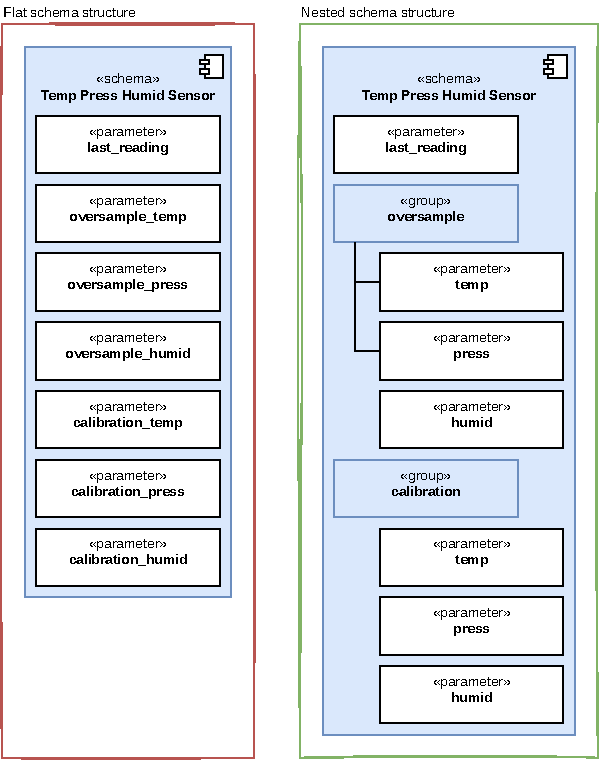
\includegraphics[width=\textwidth]{requirements_nested_configuration_groups}
    \caption{Flat schema structure (left-hand side) and Nested schema structure (right-hand side)}
    \label{fig:evaluation:requirements:nested_configuration_groups}
\end{figure}

\section{Typed Configuration Parameters}
\label{sec:requirements:typed_configuration_parameters}

The types of configuration parameters must be exposed as can be seen on the right-hand side of \autoref{fig:evaluation:requirements:typed_configuration_parameters}.
This allows defining typed external \glspl{ac:api}.

If the type of a configuration parameter is not exposed as can be seen in \autoref{fig:evaluation:requirements:typed_configuration_parameters}, it can not be passed on to external \glspl{ac:api}, allowing errors to occur caused by incompatible input data.

\begin{figure}[H]
    \centering
    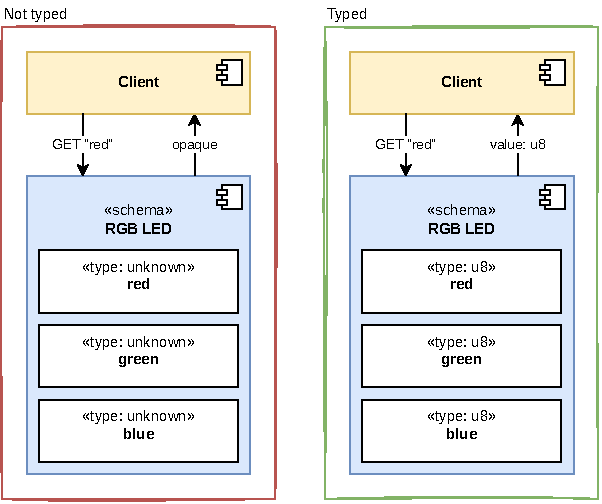
\includegraphics[width=\textwidth]{requirements_typed_configuraton_parameters}
    \caption{Not typed parameters (left-hand side) and Typed parameters (right-hand side).}
    \label{fig:evaluation:requirements:typed_configuration_parameters}
\end{figure}

\section{Binary Internal Configuration Parameter Value Format}
\label{sec:requirements:binary_internal_configuration_parameter_format}

Internally the values of the configuration parameters should be stored and passed around in their binary representation (their correct c type) as can be seen on the right-hand side of \autoref{fig:evaluation:requirements:binary_internal_configuration_parameter_format} and not converted to some inefficient format such as a string as can be seen on the left-hand side of \autoref{fig:evaluation:requirements:binary_internal_configuration_parameter_format}.

The reason for this is that strings have the following drawbacks that are especially problematic with constrained devices:

\begin{enumerate}
    \item In most cases strings consume significantly more storage than the corresponding types needed to represent the same data.

    \item Additionally, heap allocation should be avoided on constrained devices as their storage is usually small and if a program can run or not is best to be known by making sure if the binary fits on the storage or not.
          So to work with string values internally implies always storing the maximum allowed string length for each parameter, to avoid dynamic heap allocation.
          This causes an unnecessarily high amount of storage and possibly stack overhead.
          By using the concrete types, the size of each parameter is always exactly known and is never too large.

    \item Converting from- and to a string, or comparing strings causes a lot of computing overhead that can be avoided.
\end{enumerate}

\begin{figure}[H]
    \centering
    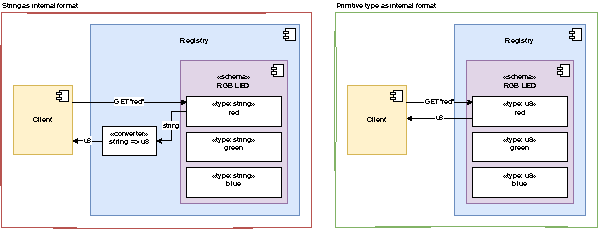
\includegraphics[width=\textwidth]{requirements_binary_internal_configuration_parameter_format}
    \caption{``String as an internal format'' (left-hand side) and Primitive type as an internal format (right-hand side).}
    \label{fig:evaluation:requirements:binary_internal_configuration_parameter_format}
\end{figure}


\section{Transactionally Commit Configuration Changes}
\label{sec:requirements:transactionally_commit_configuration_changes}

In some situations it is necessary that multiple configuration parameters change their value at the same time.
For example these configuration parameters depend on each other, such as an RGB LED that has three configuration parameters, one for red, one for green and one for blue.
If these parameters don't all change at the same time, the color of the RGB LED will not go from for example red to blue, but from red to black and then to blue or from red to pink and then to blue.
So the \gls{ac:rcs} must have the ability to fulfill this need by committing multiple configuration parameter changes in a transactional way.

\section{Persistent Configurations}
\label{sec:requirements:persistent_configurations}

Once a configuration parameter's value is changed, it muste be possible to persist this change on a non-volatile storage.
This is important because especially constrained \gls{ac:iot} devices can have power losses, for example if they are operated by solar energy.

\section{Low Implementation Effort for Modules/Drivers}
\label{sec:requirements:low_implementation_effort_for_modules_and_drivers}

The implementation effort that is necessary to get the \gls{ac:rcs} integrated into each module must be as low as possible while still fulfilling all requirements defined in this section.

If the implementation cost becomes too high, this not only makes maintainability of modules/drivers harder but lowers the chance of high adoption of this runtime configuration module into other drivers/modules in the first place.

\section{Integration with External \glspl*{gl:configuration_manager}}
\label{sec:requirements:integration_with_external_configuration_managers}

The \gls{ac:rcs} must be compatible with common external \glspl{gl:configuration_manager}.
The runtime configuration module is not supposed to specify how external configuration management works for example by introducing an official \gls{ac:coap} \gls{ac:api} but is thought of as an internal \gls{ac:api} that can be used by external \gls{gl:configuration_manager} modules that then expose this \gls{ac:api} however needed.

Currently planned external \gls{gl:configuration_manager} integrations, to which this internal
runtime configuration module must be compatible to are:

\begin{itemize}
    \item A \gls{gl:lwm2m} server \cite{oma-lwm2m-core-12}
    \item A custom \gls{ac:coap} based \gls{ac:api} \cite{RFC-7252}
    \item A custom \gls{gl:mqtt} based \gls{ac:api} \cite{mqtt311}
\end{itemize}

\chapter{Related Work}
\label{chapter:related_work}

\section{Academic Work}

\subsection{Model-driven Development of Adaptive IoT Systems}

The paper with the title ``Model-driven Development of Adaptive IoT Systems''\cite{hussein2017model} shows how to develop adaptive \gls{ac:iot} systems using a model-driven approach.
Its approach is to first model state machines of all system components using SysML4IoT \cite{7592792}, then use a publish/subscribe architecture to model the environment information and the relationship within the system.
From these state machines then the source code is generated that can be deployed to the numerous \gls{ac:iot} devices.
Those devices then change their configuration at runtime (switching to another state), if the system sends them a message that contains information that leads to a state change based on the state machine implementation.
Also the system state is synchronized with the previously designed model.
This way the system state can be manually changed by changing the state of the model.

\subsubsection{Discussion}

The approach how to handle runtime configurations of this paper is very different to our approach.
This papers designs the system as a whole first, having the relations and adaptions of the nodes in this system in mind and also providing manual runtime configuration through its model.
This creates a system that can work very well on its own, but is not very good in ``integrating with the world''.
Our goal in this thesis is to create a \gls{ac:rcs} for an operating system (\gls{gl:riot_os}), that is constructed the other way around.
Not having the final system in mind, but providing standardized \glspl{ac:api} to allow writing mappings to many standardized external \glspl{gl:configuration_manager} or protocols like \gls{gl:lwm2m}.

\subsection{Architecting Emergent Configurations in the Internet of Things}

The paper with the title ``Architecting Emergent Configurations in the Internet of Things''\cite{7930220} explains the Emergent Configurations concept and proposes an architecture for its realization.
It further focuses on how Emergent Configurations are formed to achieve user's goals and how applications can adapt to runtime context changes.
The main idea behind Emergent Configurations is that all devices integrate with each other and change their configuration / behavior depending on other devices.
The paper gives a conference room as an example, which automatically adjusts its curtains if the projector is used and depending on what kind of media is presented and if it is properly visible or not.

\subsubsection{Discussion}

The connection between this work and the \gls{ac:rcs} for \gls{gl:riot_os} is, that it shows what can be achieved when having a well designed \gls{ac:rcs}, that uses shared \glspl{ac:cs} (see \autoref{sec:requirements:shared_pre_defined_configuraiton_schemas})).
Without these stable and reliable interfaces that a shared \gls{ac:cs} offers, it would be impossible for so many different devices to communicate so flawlessly as in this paper.

\subsection{CoAP Management Interface (CORECONF)}

The paper with the title ``CoAP Management Interface (CORECONF)'' \cite{draft-ietf-core-comi-11} specifies a ``network management interface for constrained devices and networks''.
It builds on \gls{ac:coap} to access resources specified in a \gls{ac:cbor} mapping of \acrshort{ac:yang} schemas \cite{RFC-6020} and also converts the \acrshort{ac:yang} identifier string to numeric identifiers to save payload size.
If specified, \acrshort{ac:yang} schemas can have multiple instances.

\subsubsection{Discussion}

This work is similar to the requirements specified in \autoref{chapter:requirements} of our thesis, in that it uses integers as a configuration resource identifier and uses shared configuration schemas (\acrshort{ac:yang}), which support multiple instances.
The paper differs to the requirements of our thesis in that it does not specify how these configuration changes should be applied / handled by the local (constrained) device itself.
The paper only specifies a protocol for how to do configurations through the network.
The introduced CORECONF protocol can be used for external configuration management of the new \gls{gl:riot_os} \gls{ac:rcs}.

\section{Implementation Work}

\subsection{Apache Mynewt: Config}
\label{sec:analysis:related_work:mynewt_config}

Mynewt is an embedded OS developed by the Apache Software Foundation.
It is similar to \gls{gl:riot_os} and already comes with a system module for runtime configurations, called ``Config'' \cite{apache-mynewt-20}.

It manages configuration parameters as key-value pairs of strings.
A key contains a path to a configuration parameter inside a module.
For example the key ``id/serial'' means the ``serial'' parameter of the ``id'' module.
So every module that uses \gls{ac:mynewt_config}, has its own namespace (initial module name, in this case ``id'') to put configuration data and how the configuration path is structured after the namespace is defined by each module itself.
For example the ``id'' module could have a configuration parameter under the ``id/serial/i2c/instance\_1'' path.
It is also possible to optionally persist configuration values to storage, so that configurations are not lost even after a restart of a device.

\subsubsection{Internal: Handler}

Each module needs to implement a so called ``handler'' so it can expose configuration parameters to \gls{ac:mynewt_config}.
These handlers have a simple \gls{ac:api}:

\paragraph*{``ch\_get'' Function}\mbox{}

This function takes a string key as its input and returns the configuration parameter's value as a string.

\paragraph*{``ch\_set'' Function}\mbox{}

This function takes a string key and a string value as its input and sets the configuration parameters value to the given value.

\paragraph*{``ch\_commit'' Function}\mbox{}

This function takes a string key as its input, which does not need to point to a concrete configuration parameter, but could also only point to the module itself or some shorter path, because this function will be executed on every configuration parameter, that is within this path.
For example the path ``id/serial'' includes ``id/serial/i2c'' and also ``id/serial/spi''.
This function takes changes that have been previously made by calling ``ch\_set'' into effect.
Just calling ``ch\_set'' only sets a value, but does not apply it.
This way multiple configuration parameter can be set to new values one by one and then are taken into effect at the same time.

\paragraph*{``ch\_export'' Function}\mbox{}

This function takes a string key and a callback function as its input, which does not need to point to a concrete configuration parameter, but could also only point to the module itself or some shorter path, because this function will be executed on every configuration parameter, that is within this path.
For example the path ``id/serial'' includes ``id/serial/i2c'' and also ``id/serial/spi''.
This function finds all configuration parameters, that are within the given path and exports them by calling the given callback function and passing their path and their value as an argument.

\subsubsection{API}
\label{sec:related_work:mynewt_api}

The \gls{ac:api} contains of 6 basic functions, that cover the most important use cases.
It also includes a few more functions for example to help converting configuration values to and from strings, but these are not important for our thesis.

\paragraph*{Get Configuration Values}\mbox{}

It is possible to get the value of a configuration parameter by calling the ``conf\_get\_value'' function.
Internally this function finds the ``handler'' by the first element of the given path and calls its ``ch\_get'' function.

\paragraph*{Set Configuration Values}\mbox{}

It is possible to set a value of a configuration parameter to a new value by calling the ``conf\_set\_value'' function.
Internally this function finds the ``handler'' by the first element of the given path and calls its ``ch\_set'' function.

\paragraph*{Transactionally Commit Configuration Values}\mbox{}

It is possible to commit configuration parameters by calling the ``conf\_commit'' function.
Internally this function finds the ``handler'' by the first element of the given path and calls its ``ch\_commit'' function.

\paragraph*{Save Configuration Values to Storage}\mbox{}

It is possible to save configuration parameters to storage by calling the ``conf\_save'' function.
Internally this function finds the ``handler'' by the first element of the given path and calls its ``ch\_export'' function, by giving a internal function as its callback value, that then gets called by the handler's export function and writes all the configuration parameters to storage.

\paragraph*{Load Configuration Values from Storage}\mbox{}

It is possible to load configuration parameters from storage by calling the ``conf\_load'' or ``conf\_load\_one'' function.
Internally these functions look into the storage and search for either, in case of ``conf\_load\_one'', for a specific configuration parameter, or in case of ``conf\_load'', for all available configuration parameters.
For each parameter, that is found in storage, the ``conf\_set\_value'' function is then called.

\subsection{Zephyr: Settings}

Zephyr is one of the most popular current IoT operating systems.
It is part of the Linux Foundation and backed by large companies such as Google, Meta, Intel and others \cite{zephyr-20}.
Given its huge success, it is interesting to see how this rather large competitor handles runtime configuration.
The system module responsible for runtime configuration within the Zephyr operating system is called Zephyr Settings \cite{zephyr_settings_pull_request} and an implementation of \gls{ac:mynewt_config} \cite{apache-mynewt-20}.
Both \glspl{ac:api} are mostly the same but have some minor differences.

Zephyr Settings vs. \gls{ac:mynewt_config} - \gls{ac:api} Comparison:

\paragraph*{Get Configuration Values}\mbox{}

\autoref{table:mynewt_vs_zephyr_read} shows the similarities between the ``get'' functions of \gls{ac:mynewt_config} and Zephyr Settings.
The only real differences besides the usage of different names being that Zephyr settings returns an integer, while \gls{ac:mynewt_config} returns a char pointer and that the Zephyr settings \gls{ac:api} does not limit itself to passing only strings, but accepts a void pointer and has an additional ``len'' parameter, containing the size of the value.

\begin{table}[H]
      \begin{tabular}{ | l | l | }
            \hline
            M. Config   & char *conf\_get\_value(char *name, char *buf, int buf\_len);
            \\ \hline
            Z. Settings & int settings\_runtime\_get(const char *name, void *data, size\_t len);
            \\
            \hline
      \end{tabular}
      \caption{M. Config vs. Z. Settings: Read}
      \label{table:mynewt_vs_zephyr_read}
\end{table}

\paragraph*{Set Configuration Values}\mbox{}

\autoref{table:mynewt_vs_zephyr_write} shows the similarities between the ``set'' functions of \gls{ac:mynewt_config} and Zephyr Settings.
The only real differences besides the usage of different names being that Zephyr settings \gls{ac:api} does not limit itself to passing only strings, but accepts a void pointer and has an additional ``len'' parameter, containing the size of the new value.

\begin{table}[H]
      \begin{tabular}{ | l | l | }
            \hline
            M. Config   & int conf\_set\_value(char *name, char *val\_str);
            \\ \hline
            Z. Settings & \begin{tabular}[l]{@{}l@{}}int settings\_runtime\_set(const char *name, const void *data,\\size\_t *len);\end{tabular}
            \\
            \hline
      \end{tabular}
      \caption{M. Config vs. Z. Settings: Write}
      \label{table:mynewt_vs_zephyr_write}
\end{table}

\paragraph*{Transactionally Commit Configuration Values}\mbox{}

\autoref{table:mynewt_vs_zephyr_apply} shows the similarities between the ``commit'' functions of \gls{ac:mynewt_config} and Zephyr Settings.
The only real differences besides the usage of different names being that Zephyr settings \gls{ac:api} uses a const parameter.

\begin{table}[H]
      \begin{tabular}{ | l | l | }
            \hline
            M. Config   & int conf\_commit(char *name);
            \\ \hline
            Z. Settings & int settings\_runtime\_commit(const char *name);
            \\
            \hline
      \end{tabular}
      \caption{M. Config vs. Z. Settings: Apply}
      \label{table:mynewt_vs_zephyr_apply}
\end{table}

\paragraph*{Load Configuration Values from Storage}\mbox{}

\autoref{table:mynewt_vs_zephyr_load} shows the similarities between the ``load'' functions of \gls{ac:mynewt_config} and Zephyr Settings.
The only real differences is the usage of different names.

\begin{table}[H]
      \begin{tabular}{ | l | l | }
            \hline
            M. Config   & int conf\_load(void);
            \\ \hline
            Z. Settings & int settings\_load(void);
            \\
            \hline
      \end{tabular}
      \caption{M. Config vs. Z. Settings: Load}
      \label{table:mynewt_vs_zephyr_load}
\end{table}

\autoref{table:mynewt_vs_zephyr_load_a_single_parameter} shows the similarities between the ``load\_one'' functions of \gls{ac:mynewt_config} and Zephyr Settings.
The only real differences besides the usage of different names being that Zephyr settings \gls{ac:api} uses a const parameter.

\begin{table}[H]
      \begin{tabular}{ | l | l | }
            \hline
            M. Config   & int conf\_load\_one(char *name);
            \\ \hline
            Z. Settings & int settings\_load\_subtree(const char *subtree);
            \\
            \hline
      \end{tabular}
      \caption{M. Config vs. Z. Settings: Load a single parameter}
      \label{table:mynewt_vs_zephyr_load_a_single_parameter}
\end{table}

\paragraph*{Save Configuration Values to Storage}\mbox{}

\autoref{table:mynewt_vs_zephyr_save} shows the similarities between the ``save'' functions of \gls{ac:mynewt_config} and Zephyr Settings.
The only real differences is the usage of different names.

\begin{table}[H]
      \begin{tabular}{ | l | l | }
            \hline
            M. Config   & int int conf\_save(void);
            \\ \hline
            Z. Settings & int settings\_save(void);
            \\
            \hline
      \end{tabular}
      \caption{M. Config vs. Z. Settings: Save}
      \label{table:mynewt_vs_zephyr_save}
\end{table}

\autoref{table:mynewt_vs_zephyr_save_a_single_parameter} shows the similarities between the ``save\_one'' functions of \gls{ac:mynewt_config} and Zephyr Settings.
The only real differences besides the usage of different names being that Zephyr settings \gls{ac:api} does not limit itself to passing only strings, but accepts a void pointer and has an additional ``len'' parameter, containing the size of the new value.

\begin{table}[H]
      \begin{tabular}{ | l | l | }
            \hline
            M. Config   & int conf\_save\_one(const char *name, char *var);
            \\ \hline
            Z. Settings & \begin{tabular}[l]{@{}l@{}}int settings\_save\_one(const char *name, const void *value,\\size\_t val\_len);\end{tabular}
            \\
            \hline
      \end{tabular}
      \caption{M. Config vs. Z. Settings: Save a single parameter}
      \label{table:mynewt_vs_zephyr_save_a_single_parameter}
\end{table}

\subsection{\gls*{gl:lwm2m} Object and Resource Registry}
\label{sec:analysis:related_work:lwm2m}

While \gls{gl:lwm2m} by itself is a protocol for external runtime configuration management and not an operating system registry, it still has some appealing aspects that are relevant to the \nameref{sec:design:riot_registry}.
Besides the fact that the \nameref{sec:design:riot_registry} is supposed to integrate external \glspl{gl:configuration_manager} such as \gls{gl:lwm2m}.
Furthermore, it is to be evaluated if an \gls{gl:lwm2m} client such as Eclipse Wakaama \cite{eclipse_wakaama} can be used as the official \gls{gl:riot_os} configuration registry.
This way \gls{gl:lwm2m} is supposed to become the standard for \gls{gl:riot_os} configuration management and other management systems count integrate with \gls{gl:lwm2m} instead of a \gls{gl:riot_os}-specific registry.

\subsubsection{Predefined and typed object definitions}

\gls{gl:lwm2m} comes with its own predefined object definitions.
Each object definition has its own unique ID, name, and other metadata and contains multiple properties (configuration parameters) that describe the object and can be read (or written) to.
The properties themselves can not contain further child properties.
So the property list of an object definition is always flat.
Each property has an ID, a name, a type such as Integer, Boolean, String etc. and other metadata.
For example, there is the object with the ID 3420.
Its name is ``LED color light'' and it has one property ``RGB value'' with the ID 1.
This property has the type String and expects a color in the RGB hex format (\#rrggbb).

\subsubsection{Multiple instances}

The \gls{gl:lwm2m} protocol allows an object definition to have multiple instances.
So multiple modules/drivers can implement the same \gls{gl:lwm2m} object or expose multiple instances of themselves that will be accessible at the same time.
For example, a smart lamp might have multiple LEDs that all expose the same interface, but should be addressed individually to enable the mixing of different colors.

\subsubsection{Integer Resource Path}

To identify a property of some object \gls{gl:lwm2m} uses a path of 3 integers.
First comes the object ID, which is the ID of the object definition.
Second comes the instance ID which is the ID of the very instance of that object, since there can be multiple instances of each object.
And last comes the property ID.

\subsection{Prior Work on \gls*{gl:riot_os}}

Before the work on this thesis started, there has already been an initial implementation of \gls{ac:mynewt_config} (see \autoref{sec:analysis:related_work:mynewt_config}) for \gls{gl:riot_os} as an open PR on its GitHub repository (see PR 10622 \cite{riot_pr_10622} and PR 10799 \cite{riot_pr_10799}).

\section{Assessment of Implementation Work on Thesis's \acrshort{ac:rcs} Requirements}
\label{sec:related_work:assessment_of_implementation_work_on_thesis_requirements}

Besides \gls{gl:riot_os} there are other operating Systems such as Zephyr \cite{zephyr-20}, that may already provide solutions for managing runtime configurations in IoT.
So to find a suitable architecture to manage runtime configurations in \gls{gl:riot_os}, it is important to evaluate, if related work already exists, that can fully satisfy all the needs listed in \autoref{chapter:requirements}.
Besides that, it is important to learn the benefits and drawbacks of related tools to then decide whether to implement an already existing architecture into \gls{gl:riot_os} or to invent a new architecture that can benefit from what was learned while evaluating the work done in competing architectures.

\subsection{Apache Mynewt Config Subsystem}
\label{sec:related_work:mynewt_config}

\subsubsection{Advantages}
\label{sec:related_work:mynewt_config_advantages}

\begin{itemize}
      \item \textbf{\acrlongpl{ac:cs} can have a deeply nested tree structure}\\
            (see \autoref{sec:requirements:nested_configuration_groups})\\
            The configuration parameter identifier of each handler is stored as a simple string key.
            This makes it possible to easily have implicit grouping by just defining a long string with multiple separators.
            Then internally common groups of multiple parameters can be processed by the configuration subsystem.

      \item \textbf{Low implementation effort for modules/drivers}\\
            (see \autoref{sec:requirements:low_implementation_effort_for_modules_and_drivers})\\
            Every module just implements a set and get function inside a handler, that has gets or returns values as strings based on the input string, which is the identifier of a configuration parameter or group.

      \item \textbf{Easy integration with some other external \glspl{gl:configuration_manager}}\\
            (see \autoref{sec:requirements:integration_with_external_configuration_managers})\\
            Some tools that can be used for external \glspl{gl:configuration_manager} such as \gls{ac:coap} and \gls{gl:mqtt} for example can just reuse the configuration parameter path strings as address or topic.
            They can be written once and don't need to be implemented for every module (handler) of the configuration subsystem.

      \item \textbf{Transactionally Commit Configuration Changes}\\
            (see \autoref{sec:requirements:binary_internal_configuration_parameter_format})\\
            \gls{ac:mynewt_config} can transactionally commit multiple configuration changes at once my calling the ``commit'' function (see \autoref{sec:related_work:mynewt_api}).

      \item \textbf{Persistent Configurations}\\
            (see \autoref{sec:requirements:binary_internal_configuration_parameter_format})\\
            \gls{ac:mynewt_config} can persistently save configuration values to a non-volatile storage device by calling the ``conf\_save'' function (see \autoref{sec:related_work:mynewt_api}).
\end{itemize}

\subsubsection{Disadvantages}

\begin{itemize}
      \item \textbf{\acrlongpl{ac:cs} are defined per module/driver}\\
            (see \autoref{sec:requirements:shared_pre_defined_configuraiton_schemas})\\
            There are no shared configuration structure definitions that can be implemented by different modules.
            Each module implements its own custom configuration structure.
            Even if there are 2 different LED drivers, that do exactly the same except they use different hardware, they have no shared code.

      \item \textbf{No support for multiple instances}\\
            (see \autoref{sec:requirements:multiple_instances_per_schema})\\
            The subsystem itself has no construct for how instances might work.
            The implementing module/driver can of course hack around this by implementing an instance group as part of the path inside the handler and then internally map it to the duplicated devices that shall be configured.
            But this is a custom solution that will only make the configuration subsystem unnecessarily complex and inconsistent.

      \item \textbf{Path to configuration parameters as string}\\
            (see \autoref{sec:requirements:integer_path_as_identifier_of_configuration_values})\\
            The identifier of a configuration parameter is a string, which supports nested groups via ``/'' separators.
            In general, the structure of this string can be totally custom per module/driver, as the modules that implement a configuration handler decide how to interpret its structure.
            This causes a lot of overhead in string deserialization and is easy to cause errors or undocumented inconsistencies.

      \item \textbf{Configuration parameters have no type information}\\
            (see \autoref{sec:requirements:typed_configuration_parameters})\\
            Everything is based on strings.
            The handler implemented by the module must convert the input string into whatever format it needs.
            And also the other way around on return.
            In that sense, a type is not needed, as the handler takes care of it with the cost of performance overhead and a more complicated \gls{ac:api} for the user.
            If there are types the user could for example know if a number is needed or a string, which can be unclear in some scenarios.
            But this is not the case with this configuration subsystem.

      \item \textbf{Configuration parameter values are stored in the string format}\\
            (see \autoref{sec:requirements:binary_internal_configuration_parameter_format})\\
            As every parameter value is returned and set as a string value, it also is necessary to persist it as a string, so that the handler could understand it when it gets read and passed to it.
            As strings in most cases use up more storage than primitive values such as numbers, this can be a problem for constrained devices with not a lot of memory.

      \item \textbf{Difficult or almost impossible integration with some other external \glspl{gl:configuration_manager}}\\
            (see \autoref{sec:requirements:integration_with_external_configuration_managers})\\
            External \glspl{gl:configuration_manager} such as \gls{gl:lwm2m} have their predefined \gls{ac:cs} structure called object models.
            There is for example an object model for a colored light bulb.
            If this external \gls{gl:configuration_manager} is integrated with the \gls{ac:mynewt_config}, it is necessary to write a mapping for each \gls{ac:mynewt_config} handler to the corresponding object model in \gls{gl:lwm2m}.
            Considering that \gls{gl:lwm2m} is not the only standard for configuration management this becomes an issue to maintain.
            Also, some other simpler \glspl{gl:configuration_manager} could depend on integer arrays as an identifier for the configuration parameter.
            Transforming a string as is used in the parameter of the \gls{ac:mynewt_config}, will always have collisions and is therefore not reliable.
\end{itemize}

\subsubsection{Conclusion}

What is needed is not a registry that is split into modules/drivers, but a registry that defines data structures that can be implemented by multiple modules/drivers to share the same interface for identical use cases.

\subsection{\gls*{gl:lwm2m} Object and Resource Registry}
\label{sec:related_work:lwm2m}

\subsubsection{Advantages}

\begin{itemize}
      \item \textbf{\acrlongpl{ac:cs} are shared between modules/drivers}\\
            (see \autoref{sec:requirements:shared_pre_defined_configuraiton_schemas})\\
            \gls{gl:lwm2m} has predefined \glspl{ac:cs} for common use cases such as \acrshort{ac:wlan} configuration \cite{oma-lwm2m-core-12} or location data \cite[p. 124]{oma-lwm2m-core-12} called object models.
            Modules/drivers can implement these object models and in this way share the same data structure across similar use-cases.

      \item \textbf{Multiple \acrlongpl{ac:si}}\\
            (see \autoref{sec:requirements:multiple_instances_per_schema})\\
            Each \gls{gl:lwm2m} object model can be implemented and instantiated by more than one model/driver.
            To identify different instances, the instance\_id is part of the integer path to access configuration parameters: Object model/instance/parameter.

      \item \textbf{Path to configuration parameter as array of 3 integers}\\
            (see \autoref{sec:requirements:integer_path_as_identifier_of_configuration_values})\\
            The path to identify a single configuration parameter consists of 3 integers:
            Object Model ID / Instance ID / Parameter ID. This way the payload for requests will not be increased only because an object model has a long name.

      \item \textbf{Configuration parameters have type information}\\
            (see \autoref{sec:requirements:typed_configuration_parameters})\\
            A configuration parameter can have multiple types:
            String, (Unsigned) Integer, Float, Boolean, Opaque, Time \cite[p. 99]{oma-lwm2m-core-12}.
            This helps the user to find out what kind of value is valid for a given configuration parameter.

      \item \textbf{Configuration parameter values can have any internal type (string, int, binary, etc.)}\\
            (see \autoref{sec:requirements:binary_internal_configuration_parameter_format})\\
            The values of configuration parameters get set in their primary type and not formatted in some higher type such as a ``string type'' for example.

      \item \textbf{Transactionally Commit Configuration Changes}\\
            (see \autoref{sec:requirements:binary_internal_configuration_parameter_format})\\
            \gls{gl:lwm2m} has the ability to set multiple configuration parameters at once.
            If they are set at once, they would also be committed at the same time.

      \item \textbf{Persistent Configurations}\\
            (see \autoref{sec:requirements:binary_internal_configuration_parameter_format})\\
            The open source \gls{gl:lwm2m} client implementation called Eclipse Wakaama \cite{eclipse_wakaama} does not come with this feature, but it is possible to implement this functionality on top of it.
\end{itemize}

\subsubsection{Disadvantages}

\begin{itemize}
      \item \textbf{\acrlongpl{ac:cs} can not have a deeply nested tree structure}\\
            (see \autoref{sec:requirements:nested_configuration_groups})\\
            More complicated object models with many configuration parameters that can be logically structured, will have some unnecessary overhead.
            A structure can still be simulated by giving names such as:
            ``group\_a/group\_b/param\_c'' as parameter names.

      \item \textbf{High implementation effort for modules/drivers}\\
            (see \autoref{sec:requirements:low_implementation_effort_for_modules_and_drivers})\\
            The open source \gls{gl:lwm2m} client implementation called Eclipse Wakaama \cite{eclipse_wakaama} has a high implementation effort for module/driver developers to integrate it.
            For instance, the example implementation in the Wakaama Repository of the \gls{gl:lwm2m} location object model \cite[p. 125]{oma-lwm2m-core-12}, which only exposes 7 values(latitude, longitude, altitude, radius, velocity, timestamp and speed), already needs 352 lines of code \cite[p. 125]{oma-lwm2m-core-12}.

      \item \textbf{Difficult to integrate with other external \glspl{gl:configuration_manager}}\\
            (see \autoref{sec:requirements:integration_with_external_configuration_managers})\\
            \gls{gl:lwm2m} is itself an external \gls{gl:configuration_manager} and not intended as a middleware that could be integrated with other external \gls{gl:configuration_manager} tools.
            As a consequence, even though possible, the integration of other configuration tools with for example the ``Eclipse Wakaama'' client \cite{eclipse_wakaama}, which already requires considerably a lot of work to integrate itself as explained earlier, is not easily done.
            Most importantly to create good external \gls{gl:configuration_manager} integrations it is important to use meta-fields such as ``name'', or ``description''.
            Those fields exist in the \gls{gl:lwm2m} Object Model Definitions \cite[p. 68]{oma-lwm2m-core-12}, but these are only known by the \gls{gl:lwm2m} Server and not part of the \gls{gl:lwm2m} client running on the \gls{gl:riot_os} node \cite{oma-lwm2m-core-12}.
            This way the client cannot expose any human-readable information of its \gls{ac:api}, except integer paths and types.
\end{itemize}

\subsubsection{Conclusion}

Other \glspl{gl:configuration_manager} should be supported also. \gls{gl:lwm2m} is difficult to integrate with other managers.
An interface between \gls{gl:riot_os} and \gls{gl:lwm2m} is needed. For example, a new system module called \nameref{sec:design:riot_registry}.

\section{Summary of Implementation Work Assessment}
\label{sec:related_work:summary}

As \autoref{fig:related_work_influences} shows, there is a lot to be learned from existing technologies.
Especially in how different their approaches to fixing similar issues are.
But not only \gls{ac:mynewt_config} but also OMA \gls{gl:lwm2m} both on their own do not satisfy the needs of a \gls{gl:riot_os}-wide registry good enough, to be implemented as a solution to the problem.

The main issue with \gls{ac:mynewt_config} is the fact that each module would need to implement the \gls{ac:cs} on its own, which results in many similar but not identical \glspl{ac:cs} inside similar modules/drivers and also prevents the integration of external \glspl{gl:configuration_manager} such as \gls{gl:lwm2m} (see \autoref{sec:related_work:mynewt_config_advantages}).
Also, the lack of type information for configuration parameters makes the integration of external \glspl{gl:configuration_manager} that rely on type information problematic.

On the other hand, the main issues with OMA \gls{gl:lwm2m} are a way too large module implementation boilerplate and the high difficulty to integrate other external configuration managers with the local \gls{gl:lwm2m} schema.

\begin{figure}[H]
      \centering
      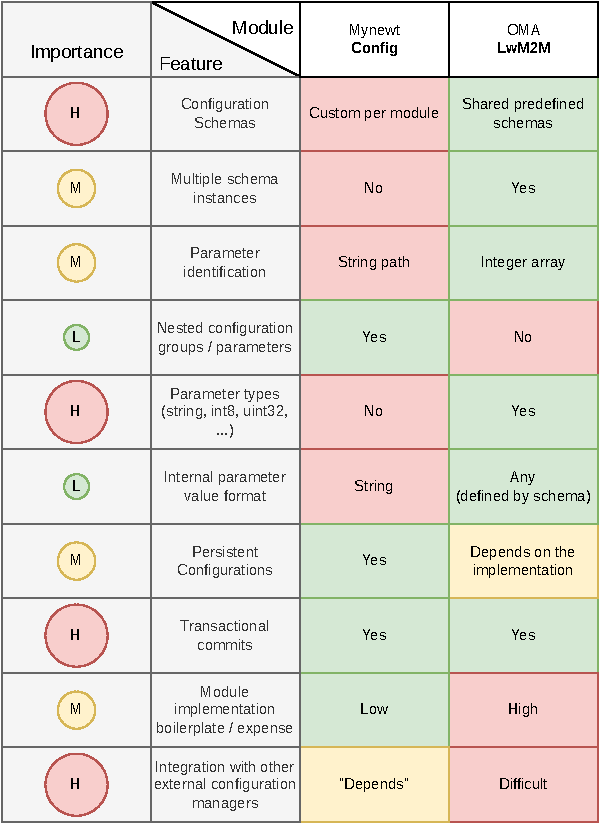
\includegraphics[width=\textwidth]{related_work_influences}
      \caption{Related work influences.}
      \label{fig:related_work_influences}
\end{figure}

\section{Conclusion of Implementation Work Assessment}
\label{sec:related_work:conclusion}

The logical consequence is the creation of a new configuration registry that is based on the concepts of \gls{ac:mynewt_config} and \gls{gl:lwm2m} but only uses those that fit the needs of the \gls{gl:riot_os} most.
It is supposed to keep the simplicity of the \gls{ac:mynewt_config}, by also supporting the advantages of OMA \gls{gl:lwm2m}.
The OMA \gls{gl:lwm2m} configuration manager can then be implemented through a mapping between the new \nameref{sec:design:riot_registry} configuration parameters and the \gls{gl:lwm2m} object models.

As can be seen on the right-hand side of \autoref{fig:related_work_conclusion}.
This new \nameref{sec:design:riot_registry} allows the specification of \glspl{ac:cs} that are shared by drivers and modules so that every driver or module that represents the same functionality will also have the same structural representation of their configuration parameters.
This also easily allows the ability to create multiple instances of the same \gls{ac:cs}.
For example, a traffic light would need 3 LEDs that use the same \gls{ac:cs}.
The identification of a configuration parameter of the \nameref{sec:design:riot_registry} is a result of its path, which is an array of integers, of which the length depends on how deeply nested the \gls{ac:cs} structure is.
To improve the integration of typed configuration managers, the configuration parameters also have metadata containing type information, but also strings such as ``name'' or ``description'' to allow the creation of more simple \glspl{ac:api} for developers.
For example a \gls{ac:cli} that allows using the name field as an alias to the integer array.
Internally the \nameref{sec:design:riot_registry} allows the \gls{ac:cs} to use every available type in the C programming language to specify the value of a configuration manager that is written to the program storage.
To prevent unnecessary conversion from string to native value and the other way around. The integration of the new registry into drivers or modules is also supposed to be as simple as possible.
Therefore, an \gls{ac:api} that is inspired by the \gls{ac:mynewt_config} (see \autoref{sec:analysis:related_work:mynewt_config}) will be implemented.

\begin{figure}[H]
      \centering
      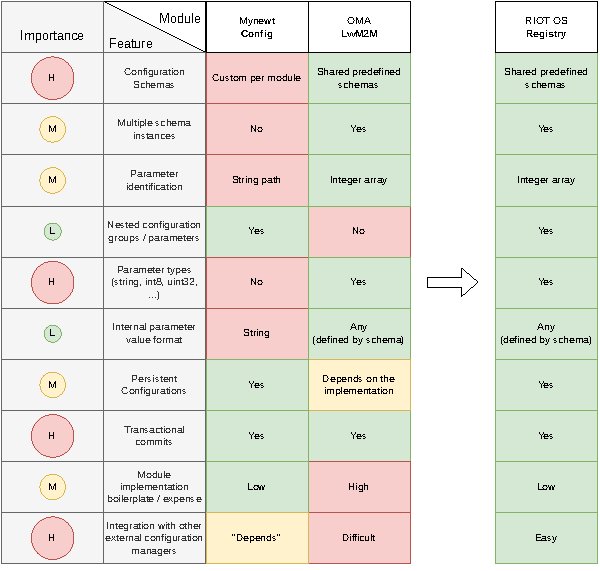
\includegraphics[width=\textwidth]{related_work_conclusion}
      \caption{Related work conclusion.}
      \label{fig:related_work_conclusion}
\end{figure}

\chapter{Design of the new RIOT OS RCS}
\label{chapter:design}

\section{Architecture}
\label{sec:design:architecture}

The proposed \gls{ac:rcs} architecture, as shown in \autoref{fig:runtime_configuration_architecture}, is formed by one or more Configuration
Managers (see \autoref{sec:design:integrating_external_configuration_managers}) and the \nameref{sec:design:riot_registry} (see \autoref{sec:design:riot_registry}).
The \nameref{sec:design:riot_registry} acts as a common interface to access Runtime Configurations and store them in non-volatile devices.
All runtime configurations can be accessed either from the \gls{gl:riot_os} application or the interfaces exposed by the \glspl{gl:configuration_manager}, via the \nameref{sec:design:riot_registry}.
A \gls{gl:riot_os} Application may interact with a \gls{gl:configuration_manager} in order to modify access control rules or enable different exposed interfaces.

\autoref{fig:runtime_configuration_architecture} shows this in more detail.
It differentiates between 2 different kinds of \glspl{gl:configuration_manager}:

\subsubsection{Basic \glspl*{gl:configuration_manager}:}
These \glspl{gl:configuration_manager} are a simple representation of the default configuration structure of the \nameref{sec:design:riot_registry}.
They only expose the parameters paths as is and do not map to any special structure.

\subsubsection{Advanced \glspl*{gl:configuration_manager}:}
These \glspl{gl:configuration_manager} have their own configuration structure (custom predefined object models etc.) and can not automatically be mapped to from the \nameref{sec:design:riot_registry} itself.
To make them work, a custom mapping module needs to be implemented, which maps each configuration parameter from the registry to the correct format of the \gls{gl:configuration_manager}.

\begin{figure}[H]
    \centering
    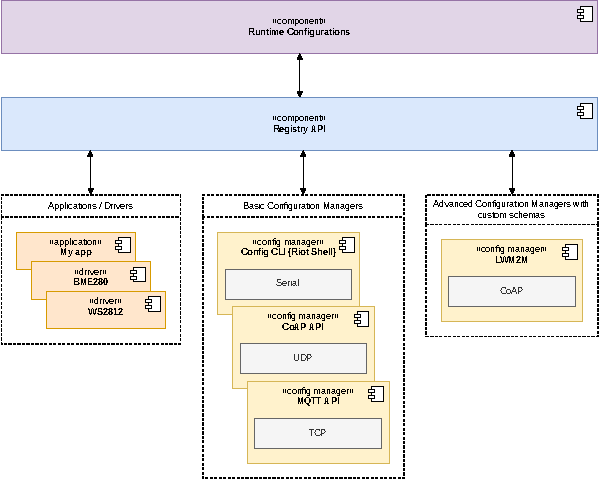
\includegraphics[width=\textwidth]{architecture}
    \caption{Runtime Configuration Architecture.}
    \label{fig:runtime_configuration_architecture}
\end{figure}

\section{\gls*{gl:riot_os} Registry}
\label{sec:design:riot_registry}

The \nameref{sec:design:riot_registry} is a module for interacting with persistent key-value configurations.
It's heavily inspired by the \gls{ac:mynewt_config} implementation and \gls{gl:lwm2m} Object Models \cite[p. 68]{oma-lwm2m-core-12}.

The \nameref{sec:design:riot_registry} interacts with \gls{gl:riot_os} modules via \glspl{ac:cs} (see \autoref{sec:design:riot_registry:configuration_schemas}), and with non-volatile storage devices via Storage Facilities (see \autoref{sec:design:riot_registry:storage_facilities}).
This way the functionality of the \nameref{sec:design:riot_registry} is independent of the functionality of a module or storage device.
It is possible to get or set the values of configuration parameters.
A \gls{ac:cp} is used to point to the correct configuration parameter.
It is also possible to transactionally apply configurations or export their values to a buffer or print them.
To persist configuration values, it is possible to store them in non-volatile storage devices.

Any mechanism of security (access control, encryption of configurations) is not directly in the scope of the Registry but in the \glspl{gl:configuration_manager} and the specific implementations of the \gls{ac:cs} and \gls{ac:sf}.

\autoref{fig:the_riot_registry_components} shows an example of two \glspl{ac:cs} (My app, LED Strip).
The application ``My app'' uses the custom ``My app'' \gls{ac:cs} to expose custom configuration parameters to the \nameref{sec:design:riot_registry} and the drivers \gls{gl:ws2812}, \gls{gl:sk6812} and \gls{gl:ucs1903} contain instances of the ``LED Strip'' \gls{ac:cs} to expose common LED Strip configuration parameters. Also, there are two Storage Facilities available:
EEPROM and FAT.

\begin{figure}[H]
    \centering
    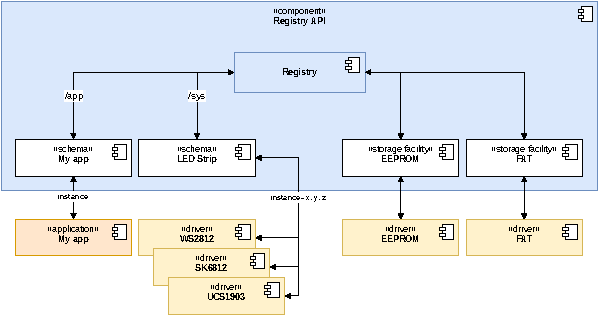
\includegraphics[width=\textwidth]{components}
    \caption{The \nameref{sec:design:riot_registry} components.}
    \label{fig:the_riot_registry_components}
\end{figure}

See Usage Flow (\autoref{sec:design:riot_registry:usage_flow}) for more information.

\subsection{\acrlong*{ac:cs} (\acrshort*{ac:cs})}
\label{sec:design:riot_registry:configuration_schemas}

A \gls{ac:cs} represents a \gls{ac:cg} in the \nameref{sec:design:riot_registry}.
A \gls{gl:riot_os} module is required to add an instance to a given \gls{ac:cs} in order to expose its configurations to the Registry \gls{ac:api}.
Or needs to implement its own custom \gls{ac:cs}.

A \gls{ac:cs} is defined by an ID, some metadata (name, description) and a get and set handler for interacting with the configuration parameters of the \gls{ac:cg}.

\begin{itemize}
    \item set: Sets a value to a configuration parameter.
    \item get: Gets the current value of a configuration parameter.
\end{itemize}

The \gls{ac:cs} also contains the struct that specifies how each instance (\gls{ac:si}) stores the actual data.

\subsubsection{\acrlong*{ac:si} (\acrshort*{ac:si})}
\label{sec:design:riot_registry:schema_instances}

An instance of a \gls{ac:cs}, which contains the actual data values.
It can be added to a \gls{ac:cs} and contains a ``commit\_cb'' handler, to notify the module containing the instance about configuration changes that need to be applied.

\begin{itemize}
    \item commit\_cb:
          To be called once configuration parameters have been set, in order to apply any further logic required to make them effective (e.g.\ handling dependencies).
\end{itemize}

\subsection{\acrlong*{ac:sf} (\acrshort*{ac:sf})}
\label{sec:design:riot_registry:storage_facilities}

An \gls{ac:sf} must implement the ``storage interface'' to allow the \nameref{sec:design:riot_registry} to load, search and store configuration parameters.
From the point of view of the \nameref{sec:design:riot_registry}, all parameters are key/value pairs with certain types, it is the responsibility of the \gls{ac:sf} to transform those into a proper format to store them.
(E.g. lines separated by a ``\textbackslash{n}'' character in a file or encoded in \gls{ac:cbor} etc.).

The interface of an \gls{ac:sf} is defined with a descriptor that has the following attributes:

\begin{itemize}
    \item load: Executes a callback function for every configuration parameter stored in the storage.

    \item store: Stores one configuration parameter in the storage.
\end{itemize}

Any kind of storage encryption mechanism is not in the scope of this document, and up to the implementation of load and store or intrinsic encryption functionalities in the storage.

A minimal \nameref{sec:design:riot_registry} setup requires at least one source \gls{ac:sf} from which configurations are loaded and exactly one \gls{ac:sf} destination to which configurations are stored.
Having multiple \gls{ac:sf} sources can be useful when it's required to migrate the data between Storage Facilities (e.g\ to migrate all configurations from \gls{ac:sf} A to B, register B as source and destination and add A as a source).

\subsection{\acrlong*{ac:cp} (\acrshort*{ac:cp})}
\label{sec:design:riot_registry:configuration_path}

A complete \gls{ac:cp} is a unique identifier of a configuration parameter.
A \gls{ac:cp} does not need to be complete and can also only point to a specific \gls{ac:cn}, \gls{ac:cs}, \gls{ac:si} or \gls{ac:cg}.
The \nameref{sec:design:riot_registry} needs this information, so that it knows where to look for the requested configuration parameter values or metadata.
Below is a regex example showing how the \gls{ac:cp} is structured.
All path elements have to be integers: ``namespace\_id/schema\_id/instance\_id/(group\_id/)*parameter\_id''.
In reality the amount of ``group\_ids'' is limited to 8 and can be changed with a `define`, so the regex is a bit simplified.

\subsubsection{\acrlong*{ac:cn} (\acrshort*{ac:cn})}
\label{sec:design:riot_registry:configuration_path_namespace}

A \gls{ac:cn} splits \glspl{ac:cs} in multiple categories. Currently specified are the following: ``SYS=0'' and ``APP=1''.
\glspl{ac:cs} that are part of ``SYS'' are \gls{gl:riot_os} internal \glspl{ac:cs} and are used to abstract common configuration structures within \gls{gl:riot_os} such as ``IEEE802154'' etc.
The ``APP'' \gls{ac:cn} must not be used by \gls{gl:riot_os} itself, but only by the application.
This is to prevent application specific \gls{ac:cs} from clashing with \gls{gl:riot_os}'s internal \gls{ac:cs}.
This is specifically important for the case of when new \glspl{ac:cs} are added in a future \gls{gl:riot_os} version.

\subsubsection{\acrlong*{ac:cg} (\acrshort*{ac:cg})}
\label{sec:design:riot_registry:configuration_path_group}

Within RIOT, each \gls{ac:si} contains a list of configuration parameters and/or \glspl{ac:cg}.
A \gls{ac:cg} can contain multiple sub-\glspl{ac:cg}.
This way a more complex \gls{ac:cs} can be split into multiple \glspl{ac:cg}, logically separating configuration parameters, instead of having them all in a flat key-value list.
Because the \nameref{sec:design:riot_registry} allows a \gls{ac:cp} to point to specific \glspl{ac:cg}, this gives the ability to do operations on a set of configuration parameters that share the same \gls{ac:cg}, without needing to address each of those configuration parameters separately.

\subsection{\acrshort*{ac:api} and Usage Flows}
\label{sec:design:riot_registry:usage_flow}

\subsubsection{\gls*{ac:api}}

\autoref{fig:riot_os_registry_api_structure} shows the \gls{ac:api} of the \nameref{sec:design:riot_registry}.
On the left-hand side the basic \gls{ac:api} to manage configuration parameters is shown.
It allows to ``set'' and ``get'' configuration parameters, transactionally ``commit'' them, ``export'' them to a buffer or terminal, ``load'' them from storage and to ``save'' them to the storage.
On the right-hand side the setup \gls{ac:api} is shown, exposing functions to register \glspl{ac:cs}, \glspl{ac:si} and \glspl{ac:sf}.

The functionality is of these functions is explained in the following paragraphs.

\begin{figure}[H]
    \centering
    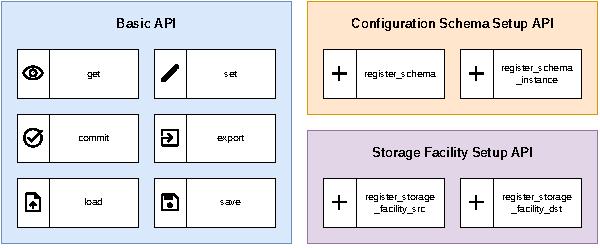
\includegraphics[width=1.0\textwidth]{api_structure}
    \caption{\nameref{sec:design:riot_registry} \gls{ac:api}.}
    \label{fig:riot_os_registry_api_structure}
\end{figure}

\subsubsection{Registry Initialization}

As described in the flow in \autoref{fig:usage_flow_of_the_riot_registry}, modules add their \glspl{ac:si} to predefined \glspl{ac:cs} or declare and register their own \gls{ac:cs} for \glspl{ac:cg} in the \nameref{sec:design:riot_registry}.
\glspl{ac:sf} are registered as sources and/or destinations of configurations in the \nameref{sec:design:riot_registry}.

\begin{figure}[H]
    \centering
    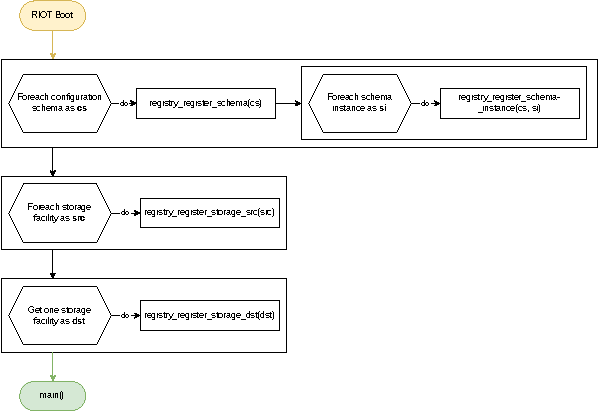
\includegraphics[width=1.0\textwidth]{behavioral_flow_boot}
    \caption{Usage flow of the \nameref{sec:design:riot_registry}.}
    \label{fig:usage_flow_of_the_riot_registry}
\end{figure}

\paragraph{Get Configurations}\mbox{}

At any time, the application or a \gls{gl:configuration_manager} can retrieve a configuration value using the (registry\_get\_value) function.

\autoref{fig:behavioral_flow_of_the_get_api} shows the flow of getting the value of a configuration parameter.
First the function ``registry\_get\_value'' is called and takes the \gls{ac:cp} as its argument.
If the registry can find the requested \gls{ac:cn}, \gls{ac:cs}, \gls{ac:si} and optionally all the \glspl{ac:cg} that are part of the \gls{ac:cp} and if the last element of the \gls{ac:cp} is a configuration parameter, then it gets its value from the \gls{ac:si} and returns it. Otherwise the error ``ENOTFOUND'' is returned.

\begin{figure}[H]
    \centering
    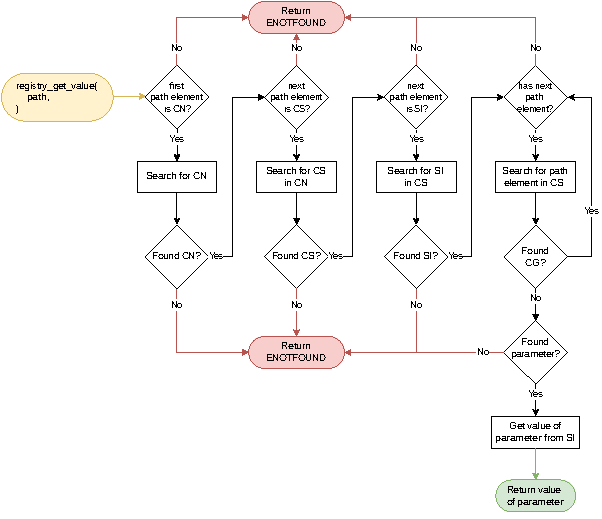
\includegraphics[width=\textwidth]{behavioral_flow_get}
    \caption{Behavioral flow of the "get" function.}
    \label{fig:behavioral_flow_of_the_get_api}
\end{figure}

\paragraph{Set Configurations}\mbox{}

At any time, the application or a \gls{gl:configuration_manager} can set a configuration value using the (registry\_set\_value) function.

\autoref{fig:behavioral_flow_of_the_set_api} shows the flow of setting a configuration parameter to a new value.
First the function ``registry\_set\_value'' is called and takes the \gls{ac:cp} as its argument.
If the registry can find the requested \gls{ac:cn}, \gls{ac:cs}, \gls{ac:si} and optionally all the \glspl{ac:cg} that are part of the \gls{ac:cp} and if the last element of the \gls{ac:cp} is a configuration parameter, then it sets its value inside the \gls{ac:si} to the new value. Otherwise the error ``ENOTFOUND'' is returned.

Note this function doesn't interact with the \gls{ac:sf}, so configuration changes are not reflected in the non-volatile storage devices unless the function ``registry\_save'' is called (see \autoref{sec:design:riot_registry:usage_flow:save_configurations_to_storage}).

\begin{figure}[H]
    \centering
    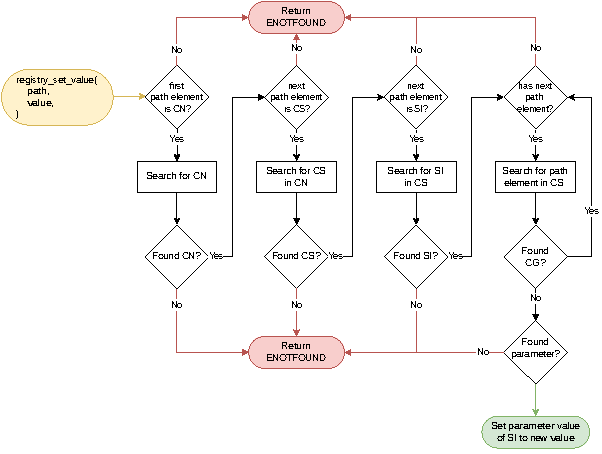
\includegraphics[width=\textwidth]{behavioral_flow_set}
    \caption{Behavioral flow of the "set" function.}
    \label{fig:behavioral_flow_of_the_set_api}
\end{figure}

\paragraph{Commit Configurations}\mbox{}
\label{sec:design:commit_configurations}

Once the value(s) of one or multiple configuration parameter(s) are changed by the ``registry\_set'' function, they still need to be committed, so that the new values are taken into effect.
At any time, the application or a \gls{gl:configuration_manager} can commit a specific, or multiple configuration value(s) using the (registry\_commit) function.

\autoref{fig:behavioral_flow_of_the_commit_api} shows this process in more detail:
First, the function ``registry\_commit'' is called and takes a \gls{ac:cp} as its argument.
If the registry can find the requested \gls{ac:cp}, each configuration parameter within this given \gls{ac:cp} will be passed on to the ``commit\_cb'' handler of the \gls{ac:si}, taking its full \gls{ac:cp} as an argument.
This callback is implemented by the modules/drivers that own the \gls{ac:si} of the currently called configuration parameter.
This way they get notified, when the configuration parameter has been committed and can apply the changes accordingly.

If the registry does not find parts of the given \gls{ac:cp}, it returns a ``ENOTFOUND'' error.

If the given \gls{ac:cp} does not point all the way to a concrete configuration parameter, but only to a \gls{ac:cn}, a \gls{ac:cs}, a \gls{ac:si} or a \gls{ac:cg}, then the registry will search for the configuration parameters of all the children of the specified \gls{ac:cp} recursively and commit them.

\begin{figure}[H]
    \centering
    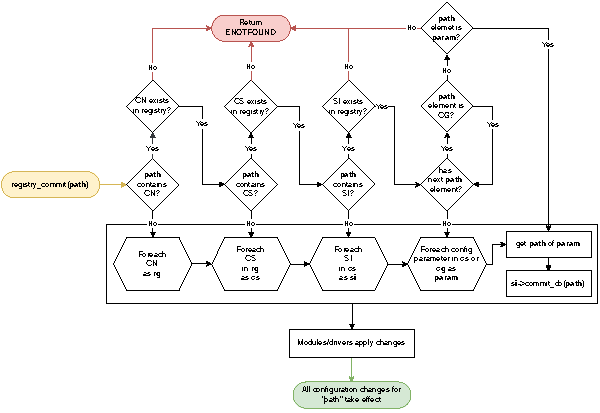
\includegraphics[width=\textwidth]{behavioral_flow_commit}
    \caption{Behavioral flow of the "commit" function.}
    \label{fig:behavioral_flow_of_the_commit_api}
\end{figure}

\paragraph{Export Configurations}\mbox{}

At any time, the application or a \gls{gl:configuration_manager} can export a specific, or multiple configuration value(s) using the (registry\_export) function.

\autoref{fig:behavioral_flow_of_the_export_api} shows the flow of exporting values and metadata of configuration parameter that are children of the given \gls{ac:cp}.
First, the function ``registry\_export'' is called and takes a \gls{ac:cp} and a ``export\_func'' callback as argument.
If the registry can find the requested \gls{ac:cp}, each configuration parameter within this given \gls{ac:cp} will be passed on to the ``export\_func'' callback, taking itself and its value as an argument, in this way exporting the configuration parameters.

If the registry does not find parts of the given \gls{ac:cp}, it returns a ``ENOTFOUND'' error.

If the given \gls{ac:cp} does not point all the way to a concrete configuration parameter, but only to a \gls{ac:cn}, a \gls{ac:cs}, a \gls{ac:si} or a \gls{ac:cg}, then the registry will search for the configuration parameters of all the children of the specified \gls{ac:cp} recursively and export them.

\begin{figure}[H]
    \centering
    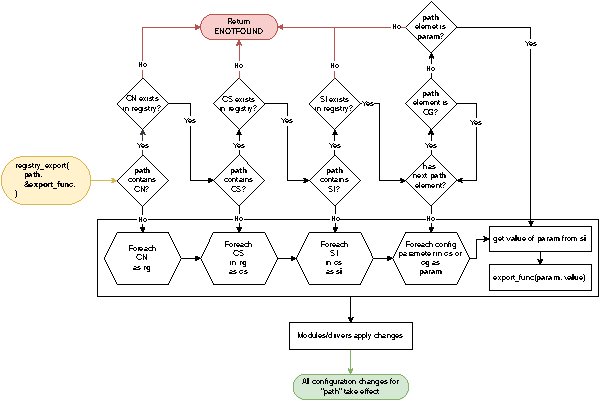
\includegraphics[width=\textwidth]{behavioral_flow_export}
    \caption{Behavioral flow of the "export" function.}
    \label{fig:behavioral_flow_of_the_export_api}
\end{figure}

\subsubsection{Load Configurations from Storage}
\label{sec:design:riot_registry:usage_flow:load_configurations_from_storage}

At any time, the application or a \gls{gl:configuration_manager} can load all configurations from the registered \gls{ac:sf} sources (registry\_load function).
For example when a device restarts after a shutdown.

\autoref{fig:behavioral_flow_of_the_load_api} shows this process in more detail:
First, the ``registry\_load'' function is called with a \gls{ac:cp} as argument, specifying which configuration parameters must be loaded from storage.
Then the ``registry\_load'' function internally calls the \gls{ac:sf}'s ``load'' handler with the storage instance, \gls{ac:cp} and the ``load\_func'' callback, which is set to the ``registry\_set\_value'' function, as arguments.
Then the \gls{ac:sf} calls the ``registry\_set\_value'' function for each configuration parameter that it finds on the storage instance's storage device.

\begin{figure}[H]
    \centering
    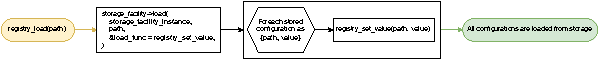
\includegraphics[width=\textwidth]{behavioral_flow_load}
    \caption{Behavioral flow of the ``load'' function.}
    \label{fig:behavioral_flow_of_the_load_api}
\end{figure}

\subsubsection{Save Configurations to Storage}
\label{sec:design:riot_registry:usage_flow:save_configurations_to_storage}

At any time, the application or a \gls{gl:configuration_manager} can store all configurations in the \gls{ac:sf} destination (registry\_save function).
For example to prevent configuration loss in case of a shutdown of the device.

\autoref{fig:behavioral_flow_of_the_save_api} shows this process in more detail:
First, the ``registry\_save'' function is called with a \gls{ac:cp} as argument, specifying which configuration parameters must be saved to storage.
Then the ``registry\_save'' function internally calls the ``registry\_export'' function with the \gls{ac:cp} and the \gls{ac:sf}'s ``save'' handler, as arguments.
Using the \gls{ac:sf}'s ``save'' handler as the export handler of the ``registry\_export'' function, causes the ``registry\_export'' function to call it for each configuration parameter, that is within the specified \gls{ac:cp} and passing its value on with it.
Then the \gls{ac:sf}'s ``save'' handler each time saves the given configuration parameter to the storage instance's storage device.

\begin{figure}[H]
    \centering
    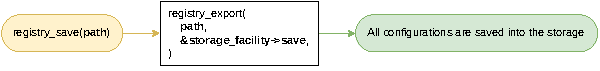
\includegraphics[width=\textwidth]{behavioral_flow_save}
    \caption{Behavioral flow of the ``save'' function.}
    \label{fig:behavioral_flow_of_the_save_api}
\end{figure}

\subsubsection{Add Custom \acrlongpl*{ac:cs} to the Registry}

The registry itself already comes with many \glspl{ac:cs} that live within the ``sys'' \gls{ac:cn}.
But sometimes an application needs some custom runtime configurations that are too specific for the registry to abstract, so it is possible to register a custom \gls{ac:cs} within the ``app'' \gls{ac:cn}.
One must not register a custom \gls{ac:cs} within the ``sys'' \gls{ac:cn}, as this is a reserved space and using it would almost certainly result in conflicts whenever \gls{gl:riot_os} gets updated.

\autoref{fig:behavioral_flow_of_the_registration_of_custom_registry_schemas} visualizes the behavioral flow of adding a custom \gls{ac:cs}:

\begin{figure}[H]
    \centering
    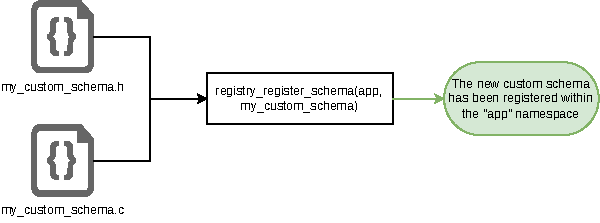
\includegraphics[width=\textwidth]{behavioral_flow_register_custom_schema}
    \caption{Behavioral flow of the registration of custom \gls{ac:cs}s.}
    \label{fig:behavioral_flow_of_the_registration_of_custom_registry_schemas}
\end{figure}

\section{Integration of External \glspl*{gl:configuration_manager}}
\label{sec:design:integrating_external_configuration_managers}

\subsection{Simple \glspl*{gl:configuration_manager}}
\label{sec:design:integrating_external_configuration_managers:simple_configuration_managers}

Simple \glspl{gl:configuration_manager} are ways to use the \nameref{sec:design:riot_registry} without the need to maintain adapters.
Those managers would only be implemented once and mirror the internal structure of the \nameref{sec:design:riot_registry}.
This can be quite powerful within \gls{gl:riot_os}-only environments, but is not as powerful in terms of its ``plug and play'' capabilities.

\subsubsection{\glsfirst*{ac:cli}}
\label{sec:design:integrating_external_configuration_managers:simple_configuration_managers:cli}

The \gls{gl:riot_os} \gls{ac:cli} can be extended with a ``registry'' command, which is followed by a sub-command ``set | get | commit | export''.\\
Each sub-command has a specific \gls{ac:cli} interface:

\begin{itemize}
    \item get: <path>
    \item set: <path> <value>
    \item commit: <path>
    \item export: <path> [-r <recursion depth>]
    \item load: [path]
    \item save: [path]
\end{itemize}

The <path> argument is a string of integers separated by ``/''.
It maps directly to the \nameref{sec:design:riot_registry} internal path structure.
The <value> argument is just the value as a string.
The ``export'' command also has the additional ``-r <recursion depth>'' flag.
It defaults to 0, which means that everything will be exported recursively.
A value of 1 means, that only the parameter that exactly matches the specified path will be exported.
A value of 2 means the same as a value of 1 but also all of its children will be exported etc.

\subsubsection{\gls*{ac:coap} \gls*{ac:api}}
\label{sec:design:integrating_external_configuration_managers:coap}

The \gls{ac:coap} \gls*{ac:api} based integration uses the \gls{gl:riot_os} internal registry structure and does not come with its own \gls{ac:cs} structure.
But \gls{ac:coap} only has a ``get'' and ``set'' function, but no ``export'' or  ``commit'' function.
So the get and set command of the \nameref{sec:design:riot_registry} will just be mapped to the get and set of \gls{ac:coap}.
For example: ``GET /namespace\_id/schema\_id/\dots'' or ``SET /namespace\_id/schema\_id/\dots -> new\_value''.
The ``export'' command can be realized through the ``GET /.well-known/core'' endpoint.
The ``commit'' command is less trivial as there is no equivalent construct within \gls{ac:coap} itself.
But here are some ideas:

\begin{itemize}
    \item Make a get request which's path has a ``commit'' prefix such as:
          ``GET /commit/namespace\_id/schema\_id/\dots''

    \item Have a dedicated ``commit'' endpoint, which can be set to a specific path, which current state will be committed on execution.
          For example: ``SET /commit -> /namespace\_id/schema\_id/\dots''.

    \item Don't implement the ``commit concept'' at all, but rather commit every ``set'' operation and allow sending values to whole \glspl{ac:cg}/\glspl{ac:cs} as their endpoint, containing values for the complete \gls{ac:cg}/\gls{ac:cs} or parts of it.
          For example in the \gls{ac:cbor} or \gls{ac:json} format.
          This way it still is possible to change multiple values at once.
\end{itemize}

\begin{figure}[H]
    \centering
    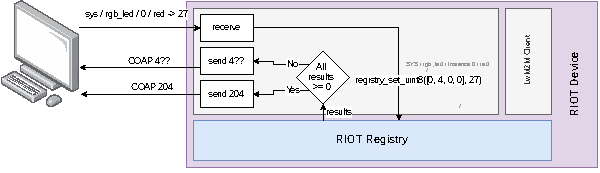
\includegraphics[width=\textwidth]{behavioral_flow_coap_integration}
    \caption{\gls{ac:coap} integration.}
    \label{fig:coap_integration}
\end{figure}

\subsubsection{\gls*{gl:mqtt} \gls*{ac:api}}

The \gls{gl:mqtt} \gls*{ac:api} based integration uses the \gls{gl:riot_os} internal registry structure and does not come with its own schema structure, but is limited to only having events with or without data.
As a consequence there are no commands such as set, get, commit or export.
Values will be set by sending a ``publish'' event containing the new value and subscribing to the same event will notify the subscriber whenever a new value is available.
This way the ``set'' and ``get'' behavior of the \nameref{sec:design:riot_registry} can be realized.
The export command is not necessary because the \gls{gl:mqtt} broker gets an initial publish for each parameter when the device boots.
So it knows about all existing topics and can expose them.
Because one \gls{gl:mqtt} broker can have multiple \gls{gl:riot_os} nodes, it is necessary to prefix the topic of each message with a device\_id.
For example: ``device\_id/namespace\_id/schema\_id/\dots''.
Less trivial is how the ``commit'' command can be exposed to \gls{gl:mqtt}. But here are some ideas:

\begin{itemize}
    \item Extend the topic of the path that needs to be committed with a ``commit'' prefix.
          For example: ``commit/device\_id/namespace\_id/schema\_id/\dots''.

    \item Have a dedicated ``commit'' topic, which can be set to a specific path, which then will be committed.
          For example:
          ``SET /commit -> /namespace\_id/schema\_id/\dots''.

    \item Don't implement the ``commit concept'' at all, but rather commit every ``set'' operation and allow sending values to whole \glspl{ac:cs}/\glspl{ac:cs} as their endpoint, containing values for the complete \gls{ac:cs}/\gls{ac:cs} or parts of it.
          For example in the \gls{ac:cbor} or \gls{ac:json} format. This way it still is possible to change multiple values at once.
\end{itemize}

\begin{figure}[H]
    \centering
    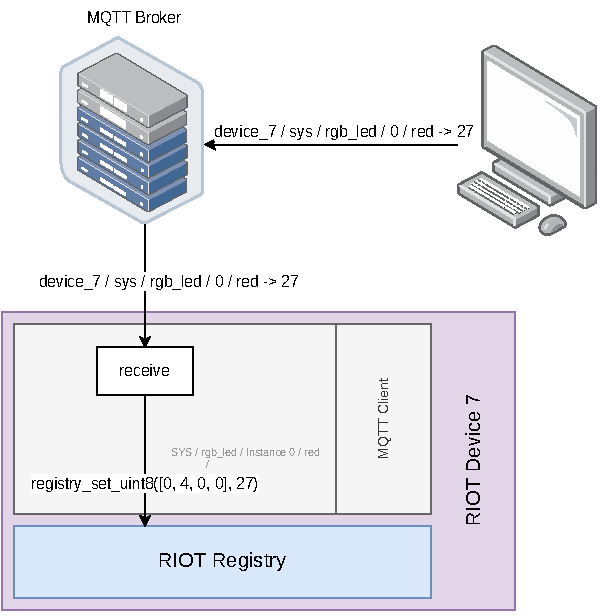
\includegraphics[width=\textwidth]{behavioral_flow_mqtt_integration}
    \caption{\gls{gl:mqtt} integration.}
    \label{fig:mqtt_integration}
\end{figure}

\subsection{Advanced \glspl*{gl:configuration_manager}}
\label{sec:design:integrating_external_configuration_managers:advanced_configuration_managers}

While having the ability to use the Registry inside \gls{gl:riot_os} and using a (\acrshort{ac:uart}) \gls{ac:cli}, the registry itself is designed so that it can easily integrate with common external \glspl{gl:configuration_manager}.
This makes it possible to modify parameters for example via the Ethernet, LoRa, Bluetooth, 802.15.4 etc.
The basic idea is that the \nameref{sec:design:riot_registry} with its predefined \glspl{ac:cs} defines a \gls{gl:riot_os} internal specification, as to which kind of data is to be found where.
Then each external \gls{gl:configuration_manager} has to implement its adapter module, which maps/converts its data structures to the \nameref{sec:design:riot_registry}.

\subsubsection{\gls*{gl:lwm2m}}

\gls{gl:lwm2m} is a relatively new protocol that is similar to the \nameref{sec:design:riot_registry} in that it specifies official (and unofficial) so-called ``object models'' that define which information can be found where.
It internally uses \gls{ac:coap} and has a concept of instances as well.
A typical \gls{gl:lwm2m} configuration parameter identifier/path has the following structure:
``object\_id/instance\_id/parameter\_id''.
The ``object\_id'' is similar to \gls{gl:riot_os}'s ``schema\_id'', the ``instance\_id'' is the same as in \gls{gl:riot_os} and the ``parameter\_id'' is also the same as in \gls{gl:riot_os} except \gls{gl:lwm2m} does not know anything about nesting, so there are no paths longer than `3` \cite{oma-lwm2m-core-12}.
To integrate \gls{gl:lwm2m} into the \nameref{sec:design:riot_registry} it is necessary to write an adapter that maps the \gls{gl:lwm2m} object models to the \nameref{sec:design:riot_registry} \glspl{ac:cs}.
An example of how this adapter would handle a ``set'' operation can be seen below:

\begin{figure}[H]
    \centering
    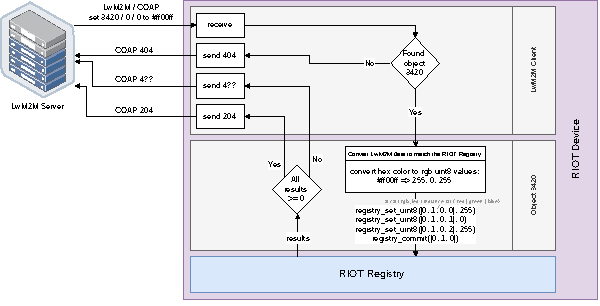
\includegraphics[width=\textwidth]{behavioral_flow_lwm2m_integration}
    \caption{\gls{gl:lwm2m} integration.}
    \label{fig:lwm2m_integration}
\end{figure}

\chapter{Implementation of the \nameref*{sec:design:riot_registry}}
\label{chapter:implementation}

This chapter shows the implementation details of \autoref{chapter:design}.
The full source code is on the enclosed CD and on GitHub \footnote{\url{https://github.com/LasseRosenow/riot-runtime-config}}.

\section{\glsfirst*{ac:cs}}

This section shows the implementation details of the in \autoref{sec:design:riot_registry:configuration_schemas} specified \glspl{ac:cs}.
The ``sys''-\gls{ac:cn} \glspl{ac:cs} are implemented in an additional module called ``registry\_schemas''.
By default every \gls{ac:cs}, that is implemented inside that module is disabled, because those implementations are depending on CFLAGS to be set.
The structure of those CFLAGS is the following:
``DCONFIG\_REGISTRY\_ENABLE\_SCHEMA\_\{schema\_name\}'', where ``{schema\_name\}'' must be replaced with the name of an existing \gls{ac:cs} such as ``RGB\_LED'' or ``FULL\_EXAMPLE''.

\autoref{fig:riot_registry_schema_structure} shows the structure of a \gls{ac:cs}.
It consists of an id, which is used in the \gls{ac:cp}, a name and description metadata field so that \glspl{gl:configuration_manager} can provide a less confusing interface, a list of \glspl{ac:si} and an items field, which contains an array of ``Schema Items''.
The list of \glspl{ac:si} needs to be stored in the \gls{ac:cs} because the \nameref{sec:design:riot_registry} is supposed to do avoid dynamic heap allocation (see \autoref{sec:requirements:binary_internal_configuration_parameter_format}). This list is a linked list, so every newly registered \gls{ac:si} will be added at the end of the list.
The Schema Items of the items field represent either a configuration parameter or a \gls{ac:cg}. Each Schema Item has a Registry ID as well as a name and a description metadata field. If a Schema Item is a \gls{ac:cg}, then it contains an array of Schema items as its value union field. Otherwise it contains a configuration parameter type of the concrete type ``Registry Type''.

Besides its fields the \gls{ac:cs} also contains a callback function inside its ``mapping'' field.
This function translates a configuration parameter ID to a pointer of the configuration parameter's value inside the \gls{ac:si}.
It also returns the size of this configuration parameter value.
This function is necessary because how a \gls{ac:si} stores its data is decided by each \gls{ac:cs}'s implementation. So only the \gls{ac:cs} knows how to translate between a configuration parameter ID and the actual data location inside the \gls{ac:si}.

\begin{figure}[H]
    \centering
    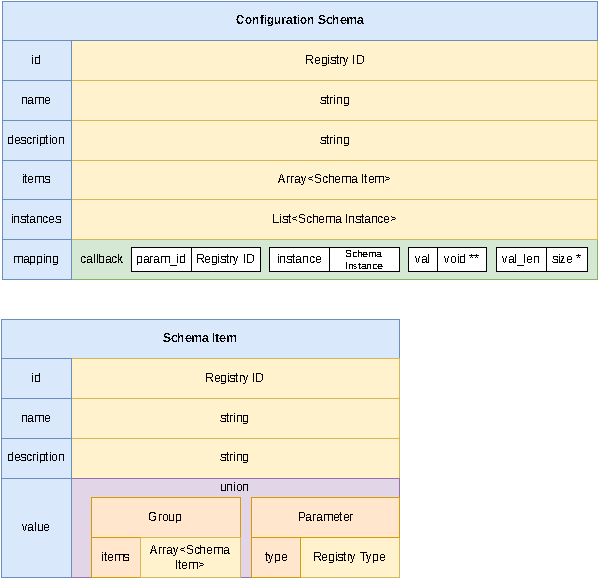
\includegraphics[width=\textwidth]{data_structure_schema}
    \caption{\nameref{sec:design:riot_registry} \gls{ac:cs} implementation data structure.}
    \label{fig:riot_registry_schema_structure}
\end{figure}

\autoref{fig:riot_registry_configuration_parameter_type_enum} shows the data structure of the ``Registry Type'' type.
A Registry Type is an enum that can be either of type ``none'', if the type is not known.
This is usually used to show, that something went wrong or as a placeholder for as long as a type is not yet known.
It can also have the type ``opaque''.
This is used to allow the \nameref{sec:design:riot_registry} to support every other type of data that does not fit into one of the other types.
It internally has the void pointer type and a specified size.
Additionally a string of a fixed size, a boolean, a uint8, a uint16, a uint32, a uint64, a int8, a int16, a int32, a int64, a float32 and a float64 are supported as a Registry Type.

\begin{figure}[H]
    \centering
    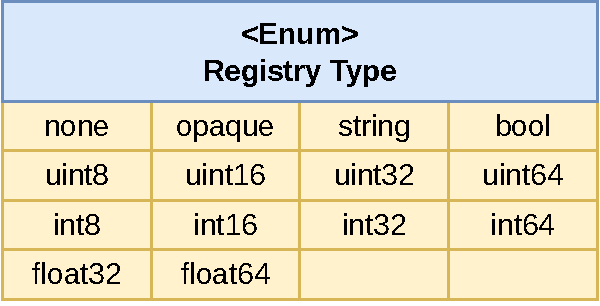
\includegraphics[width=0.5\textwidth]{data_structure_registry_type}
    \caption{\nameref{sec:design:riot_registry} configuration parameter type implementation enum.}
    \label{fig:riot_registry_configuration_parameter_type_enum}
\end{figure}

\autoref{fig:riot_registry_schema_instance_structure} shows the data structure of a \gls{ac:si}.
The ``name'' field allows it \gls{ac:si} to have a human readable soft identifier.
The ``data'' field contains its configuration parameter values in whatever format the \gls{ac:cs} implementation decides on.
The ``commit\_cb'' callback function is called whenever a configuration parameter's new value of this \gls{ac:si} gets ``committed'' (see \autoref{sec:design:commit_configurations}).
This way the module or driver that holds this \gls{ac:si} can apply the configuration parameter changes inside the ``commit\_cb'' function.


\begin{figure}[H]
    \centering
    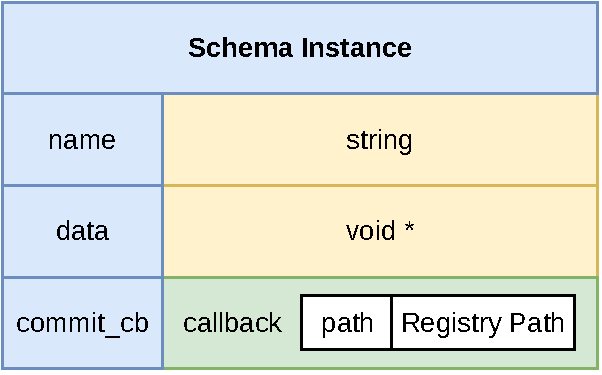
\includegraphics[width=0.5\textwidth]{data_structure_schema_instance}
    \caption{\nameref{sec:design:riot_registry} \gls{ac:si} implementation data structure.}
    \label{fig:riot_registry_schema_instance_structure}
\end{figure}

\autoref{lst:registry_schemas_h} shows the header file of the ``registry\_schemas'' module with an example RGB LED \gls{ac:cs}.
In line 4 the ``registry\_schema\_init'' function is defined, which registers all enabled ``sys''-\gls{ac:cn} \glspl{ac:cs} at the \nameref{sec:design:riot_registry}.
From line 7 - 10 is an enum that defines which \gls{ac:cs} gets which ID.
This enum prevents that two \glspl{ac:cs} use the same ID.
In line 13 the \gls{ac:cs} variable is created which will be implemented in the corresponding C file.
Line 16 - 21 is the struct definition of a \gls{ac:si}. For a RGB LED \gls{ac:cs} a red, green and blue uint8 value is enough.
In line 24 - 28 the configuration parameter IDs are set using an enum again.
These will be used in the C file, when implementing the \gls{ac:cs}.

\begin{lstlisting}[
    language=c,
    caption={Example \gls{ac:cs} implementation: registry\_schemas.h},
    label={lst:registry_schemas_h}
]
#include "registry.h"

/* initialize schemas */
void registry_schemas_init(void);

/* schema IDs */
typedef enum {
    REGISTRY_SCHEMA_RGB_LED      = 1,
    /* SOME_OTHER_SCHEMA         = 2, ... */
} registry_schema_id_t;

/* RGB LED schema */
extern registry_schema_t registry_schema_rgb_led;

/* RGB LED instance */
typedef struct {
    clist_node_t node;
    uint8_t red;
    uint8_t green;
    uint8_t blue;
} registry_schema_rgb_led_t;

/* RGB LED configuration parameter IDs */
typedef enum {
    REGISTRY_SCHEMA_RGB_LED_RED,
    REGISTRY_SCHEMA_RGB_LED_GREEN,
    REGISTRY_SCHEMA_RGB_LED_BLUE,
} registry_schema_rgb_led_indices_t;
\end{lstlisting}

\autoref{lst:registry_schemas_init_c} shows the source code of the ``registry\_schema\_init.c'' file.
In this C file, the ``registry\_schemas\_init'' function is implemented.
In line 6 it is checked if the ``CONFIG\_REGISTRY\_ENABLE\_SCHEMA\_RGB\_LED'' flag to enable the RGB LED \gls{ac:cs} is set.
If the flag is set, then in line 7 - 10 the RGB LED \gls{ac:cs} gets registered in the \nameref{sec:design:riot_registry}.
As the RGB LED schema is supposed to be a ``sys''-\gls{ac:cn} \gls{ac:cs}, the \gls{ac:cn} is set to 0 using the ``REGISTRY\_ROOT\_GROUP\_SYS'' enum value.
In line 9 the in \autoref{lst:registry_schemas_h} defined \gls{ac:cs} variable is passed as an argument.

\begin{lstlisting}[
    language=c,
    caption={Example \gls{ac:cs} implementation: registry\_schemas\_init.c},
    label={lst:registry_schemas_init_c}
]
#include "registry.h"
#include "registry_schemas.h"

void registry_schemas_init(void)
{
    if (IS_ACTIVE(CONFIG_REGISTRY_ENABLE_SCHEMA_RGB_LED)) {
        registry_register_schema(
            REGISTRY_ROOT_GROUP_SYS,
            &registry_schema_rgb_led,
        );
    }
}
\end{lstlisting}

\autoref{lst:registry_schema_rgb_led_c} shows the source code of the ``registry\_schema\_rgb\_led.c'' file. It contains an example RGB LED \gls{ac:cs} implementation.
To create a \gls{ac:cs}, the ``REGISTRY\_SCHEMA'' macro can be used as seen in line 3.
This macro takes the in \autoref{lst:registry_schemas_h} defined \gls{ac:cs} variable, the \gls{ac:cs} ID, 2 strings and a ``mapping'' function as its arguments.
Additionally as can be seen from line 9 - 19, it can take infinitely more configuration parameter macros (``REGISTRY\_PARAMETER\_*'') or \gls{ac:cg} macros (``REGISTRY\_GROUP'') as its arguments. The latter not being present in this example.
With these values, the macros generate a struct of the structure explained in \autoref{fig:riot_registry_schema_structure}.
In line 6 as an example, the first string will be the value of the name field and the second string will be the value of the description filed of the \gls{ac:cs} struct.
Line 23 to line 47 show the ``mapping'' function implementation.
In line 29 this function casts the data field of the \gls{ac:si} to the correct struct of this \gls{ac:cs}'s implementation.
From line 31 to 46, depending on which configuration parameter ID is provided, the output pointer of a pointer (``val'') gets set to the pointer of the \gls{ac:si}'s value. An example of this can be seen in line 33. The second output pointer's value (``val\_len'') gets set to the size of the configuration parameter's value. An example of this can be seen in line 34.

\begin{lstlisting}[
    language=c,
    caption={Example \gls{ac:cs} implementation: registry\_schema\_rgb\_led.c},
    label={lst:registry_schema_rgb_led_c}
]
#include "registry_schemas.h"

REGISTRY_SCHEMA(
    registry_schema_rgb_led,
    REGISTRY_SCHEMA_RGB_LED,
    "rgb", "Representation of an rgb color.",
    mapping,

    REGISTRY_PARAMETER_UINT8(
        REGISTRY_SCHEMA_RGB_LED_RED,
        "red", "Intensity of the red color of the rgb lamp.")

    REGISTRY_PARAMETER_UINT8(
        REGISTRY_SCHEMA_RGB_LED_GREEN,
        "green", "Intensity of the green color of the rgb lamp.")

    REGISTRY_PARAMETER_UINT8(
        REGISTRY_SCHEMA_RGB_LED_BLUE,
        "blue", "Intensity of the blue color of the rgb lamp.")

    );

static void mapping(
    const registry_id_t param_id,
    const registry_instance_t *instance,
    void **val,
    size_t *val_len,
) {
    registry_schema_rgb_led_t *_instance = (registry_schema_rgb_led_t *)instance->data;

    switch (param_id) {
    case REGISTRY_SCHEMA_RGB_LED_RED:
        *val = &_instance->red;
        *val_len = sizeof(_instance->red);
        break;

    case REGISTRY_SCHEMA_RGB_LED_GREEN:
        *val = &_instance->green;
        *val_len = sizeof(_instance->green);
        break;

    case REGISTRY_SCHEMA_RGB_LED_BLUE:
        *val = &_instance->blue;
        *val_len = sizeof(_instance->blue);
        break;
    }
}
\end{lstlisting}

\autoref{lst:example_cs_main_c} shows an example application that uses the RGB LED \gls{ac:cs}.
From line 5 - 25 the \gls{ac:si} callback function is implemented.
In this implementation this function only prints the \gls{ac:cn}, \gls{ac:cs} and \gls{ac:si} of the committed \gls{ac:cp}, if the \gls{ac:cp} parameter ``path'' provides these values.
From line 28 - 32 a variable that initializes an RGB LED \gls{ac:si} struct, giving default values to the red, green and blue fields.
From line 35 - 39 a variable is defined, initializing a \nameref{sec:design:riot_registry} \gls{ac:si} struct.
This struct takes the callback function of line 5 and the RGB LED \gls{ac:si} struct as its value.
In line 44 the registry gets initialized by calling the ``registry\_init'' function.
Then in line 47 the \glspl{ac:cs} get initialized by calling the ``registry\_schemas\_init'' function. And finally from line 50 - 54 the \nameref{sec:design:riot_registry} \gls{ac:si} struct that got initialized in line 35, is registered in the \nameref{sec:design:riot_registry} using the ``registry\_register\_schema\_instance'' function, providing the ``sys'' \gls{ac:cn} and the id of the \gls{ac:cs} as additional arguments.

\begin{lstlisting}[
    language=c,
    caption={Example \gls{ac:cs} implementation: main.c},
    label={lst:example_cs_main_c}
]
#include "registry.h"
#include "registry_schemas.h"

/* schema instance commit callback */
int rgb_led_instance_0_commit_cb(
    const registry_path_t path,
    const void *context,
) {
    (void)context;

    /* print CN, CS ID and SI ID if available */
    printf("RGB instance commit_cb was executed: %d", *path.namespace_id);
    
    if (path.schema_id) {
        printf("/%d", *path.schema_id);
    }

    if (path.instance_id) {
        printf("/%d", *path.instance_id);
    }
    
    printf("\n");
    
    return 0;
}

/* schema instance data struct */
registry_schema_rgb_led_t rgb_led_instance_0_data = {
    .red = 0,
    .green = 255,
    .blue = 70,
};

/* schema instance */
registry_instance_t rgb_led_instance_0 = {
    .name = "rgb-0",
    .data = &rgb_led_instance_0_data,
    .commit_cb = &rgb_led_instance_0_commit_cb,
};

int main(void)
{
    /* init registry */
    registry_init();

    /* init schemas */
    registry_schemas_init();

    /* register schema instance */
    registry_register_schema_instance(
        REGISTRY_NAMESPACE_SYS,
        registry_schema_rgb_led.id,
        &rgb_led_instance_0,
    );

    return 0;
}
\end{lstlisting}

\section{\glsfirst*{ac:sf}}

This section shows the implementation details of the in \autoref{sec:design:riot_registry:storage_facilities} specified \glspl{ac:sf}.
The \nameref{sec:design:riot_registry} comes with a few officially supported \glspl{ac:sf} implemented in the ``registry\_storage\_facilities'' module.
By default every \gls{ac:sf}, that is implemented inside that module is disabled, because those implementations are depending on CFLAGS to be set.
The structure of those CLFAGS is the following: ``DCONFIG\_REGISTRY\_ENABLE\_STORAGE\_FACILITY\_\{storage\_facility\_name\}”'', where ``\{storage\_facility\_name\}'' must be replaced with the name of an existing \gls{ac:sf} such as ``VFS''.

\autoref{fig:riot_registry_storage_facility_structure} shows the structure of a \gls{ac:sf}.
It consists of four callback functions.
A ``load'' callback function that both take a ``Storage Facility Instance'', a \gls{ac:cp} and another callback as its arguments.
Inside the load function the \gls{ac:sf} searches for configuration parameter values of the given \gls{ac:cp}.
Therefor it might need for example a filesystem mount.
This is specified in the data field of the ``Storage Facility Instance'' as a void pointer.
The callback argument of the load callback takes a \gls{ac:cp} and a ``Registry Value'' as an argument.
This callback gets executed on every configuration parameter that is found and matches the provided \gls{ac:cp}.
The \nameref{sec:design:riot_registry} sets this callback to the ``registry\_value\_set'' function.
Besides the ``load'' callback function, the \gls{ac:sf} struct also has a ``save\_start'' and a ``safe\_end'' callback function.
Both take the ``Storage Facility Instance'' as an argument.
The ``save\_start'' callback function gets called before the ``save'' callback function gets executed and is used to initialize the storage device, for example to mount a filesystem before multiple save operations are executed.
This way unnecessary overhead of continuously mounting and unmounting filesystems can be avoided.
The ``save\_end'' callback function gets called after the ``save'' function finished its execution and is used to teardown the storage device, for example unmount a filesystem, after all ``save'' operations are completed.
The ``save'' callback function takes a ``Storage Facility Instance'', a \gls{ac:cp} and a ``Registry Value'' as its arguments.
It saves the provided configuration parameter value (Registry Value) on the storage, in a by the \gls{ac:sf} defined structure, so that the ``load'' function can find it by its \gls{ac:cp}.

\begin{figure}[H]
    \centering
    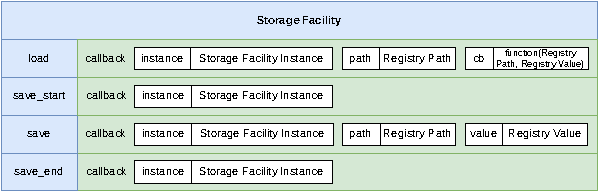
\includegraphics[width=\textwidth]{data_structure_storage_facility}
    \caption{\nameref{sec:design:riot_registry} \gls{ac:sf} implementation data structure.}
    \label{fig:riot_registry_storage_facility_structure}
\end{figure}

\autoref{fig:riot_registry_storage_facility_instance_structure} shows the structure of a \gls{ac:sf} Instance.
It holds a pointer to a \gls{ac:sf} implementation and provides data such as a filesystem mount as a void pointer.

\begin{figure}[H]
    \centering
    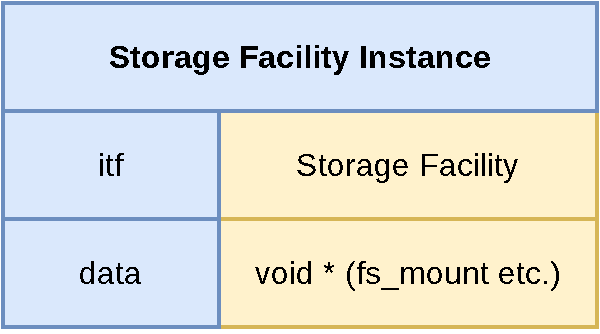
\includegraphics[width=0.44\textwidth]{data_structure_storage_facility_instance}
    \caption{\nameref{sec:design:riot_registry} \gls{ac:sf} Instance implementation data structure.}
    \label{fig:riot_registry_storage_facility_instance_structure}
\end{figure}

\autoref{fig:riot_registry_configuration_parameter_value} shows the structure of a configuration parameter called ``Registry Value''.
It has a ``type'' field which specifies the primitive type of the configuration parameter's value.
Its value is then stored in the ``buf'' field, which has a void pointer as its type.
To pass the buffer around the program safely, it is also important to know its size, so there is a third field with the name ``buf\_len'', which holds the size of the value, stored in the ``buf'' field.

\begin{figure}[H]
    \centering
    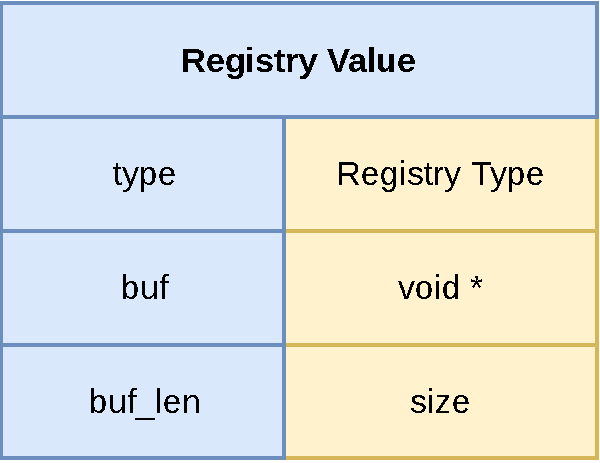
\includegraphics[width=0.4\textwidth]{data_structure_registry_value}
    \caption{\nameref{sec:design:riot_registry} configuration parameter value implementation structure.}
    \label{fig:riot_registry_configuration_parameter_value}
\end{figure}

\autoref{lst:registry_storage_facilities_h} shows the header file of the ``registry\_storage\_facilities'' module.
It contains an example ``VFS'' \gls{ac:sf} variable definition called ``registry\_storage\_facility\_vfs''.

\begin{lstlisting}[
    language=c,
    caption={Example \gls{ac:sf} implementation: registry\_storage\_facilities.h},
    label={lst:registry_storage_facilities_h}
]
#include "registry.h"

/* vfs storage facility instance */
extern registry_storage_facility_t registry_storage_facility_vfs;
\end{lstlisting}

\autoref{lst:registry_storage_facilitiy_vfs_c} shows the implementation of the VFS \gls{ac:sf}.
Because the full VFS \gls{ac:sf} implementation is around 400 lines of code, the provided \gls{ac:sf} source code in this thesis is reduced.
The full source code is on the enclosed CD and on GitHub \footnote{\url{https://github.com/LasseRosenow/riot-runtime-config/blob/main/external_modules/registry_storage_facilities/storage_facility_vfs.c}}.
In line 23 - 26 the \gls{ac:sf} variable is initialized and the load and save callback functions are taken as arguments.
The ``save'' function of the VFS \gls{ac:sf} creates a folder for every \gls{ac:cn} if it does not exist yet. It also creates a folder for every \gls{ac:cs} ID inside its \gls{ac:cn} folder. The same goes for the \gls{ac:si} ID, and the \gls{ac:cg} IDs. For the configuration parameters it does not create a folder, but create a file that also uses its ID as its filename.
Inside the file the configuration parameters value is written as binary.
The ``load'' function of the VFS \gls{ac:sf} scans the storage for folders and files that match the provided \gls{ac:cp}.
If those files match the \gls{ac:cp}, it asks the \nameref{sec:design:riot_registry} for the metadata of the configuration parameter by calling the ``registry\_get\_value'' function.
This way it can find out the correct size of the configuration parameters value and reads it from the storage.
This value is then returned using the provided callback function.

\begin{lstlisting}[
    language=c,
    caption={Example \gls{ac:sf} implementation: registry\_storage\_facility\_vfs.c},
    label={lst:registry_storage_facilitiy_vfs_c}
]
#include "registry_storage_facilities.h"

/* load data from storage */
static int load(
    const registry_storage_facility_instance_t *instance,
    const registry_path_t path,
    const load_cb_t cb,
    const void *cb_arg,
) {
    /* Loop through storage and call "load_cb_t" on each configuration parameter that is compatible to the specified path. */
}

/* save data to storage */
static int save(
    const registry_storage_facility_instance_t *instance,
    const registry_path_t path,
    const registry_value_t value
) {
    /* Open the file under the specified path and write the new value inside. */
}

/* storage facility */
registry_storage_facility_t registry_storage_facility_vfs = {
    .load = load,
    .save = save,
};
\end{lstlisting}

\autoref{lst:example_sf_main_c} shows the source code of an example application using the VFS \gls{ac:sf}.
From line 6 - 14 the filesystem mount is being configured.
Then in line 17 - 26 the VFS \gls{ac:sf} Instance is created, which takes the filesystem mount and the \gls{ac:sf} (``registry\_storage\_facility\_vfs'') as its field's values.
Then from line 28 - 38 the main function of the program is implemented.
First in line 31 the \nameref{sec:design:riot_registry} is initialized by calling the ``registry\_init'' function.
Then in line 34 the source \gls{ac:sf} is registered in the \nameref{sec:design:riot_registry} by calling the ``registry\_register\_storage\_facility\_src'' function. And finally in line 35 the destination \gls{ac:sf} is registered in the \nameref{sec:design:riot_registry} by calling the ``registry\_register\_storage\_facility\_dst'' function.

\begin{lstlisting}[
    language=c,
    caption={Example \gls{ac:sf} implementation: main.c},
    label={lst:example_sf_main_c}
]
#include "registry.h"
#include "registry_storage_facilities.h"
#include "fs/littlefs2_fs.h"

/* initialize vfs mount */
static littlefs2_desc_t fs_desc = {
    .lock = MUTEX_INIT,
};

static vfs_mount_t vfs_mount = {
    .fs = &FS_DRIVER,
    .mount_point = "/sda",
    .private_data = &fs_desc,
};

/* initialize a storage facility source instance */
registry_storage_facility_instance_t vfs_instance_src = {
    .itf = &registry_storage_facility_vfs,
    .data = &vfs_mount,
};

/* initialize a storage facility destination instance */
registry_storage_facility_instance_t vfs_instance = {
    .itf = &registry_storage_facility_vfs,
    .data = &vfs_mount,
};

int main(void)
{
    /* init registry */
    registry_init();

    /* register storage_facility source and destination instances */
    registry_register_storage_facility_src(&vfs_instance_src);
    registry_register_storage_facility_dst(&vfs_instance_dst);

    return 0;
}
\end{lstlisting}

\section{\glsfirst*{ac:cp}}

This section shows the implementation details of the in \autoref{sec:design:riot_registry:configuration_path} specified \gls{ac:cp}.

\autoref{fig:riot_registry_path_structure} shows the structure of the \gls{ac:cp} on the left-hand side.
It contains a \gls{ac:cn} field, that is implemented as an enum containing a ``sys''=0 and a ``app''=1 value as possible \glspl{ac:cn}.
The \gls{ac:cp} also has a \gls{ac:cs} ID field, which is of the type ``Registry ID''.
The Registry ID type internally is a uint32 type.
The \gls{ac:cp} also has a field that holds the \gls{ac:si} ID, which is also of the Registry ID type.
And at last the \gls{ac:cp} has a ``path'' field, which is an array of ``Registry IDs''.
The ``path'' field contains the \gls{ac:cg} and configuration parameter IDs.

\begin{figure}[H]
    \centering
    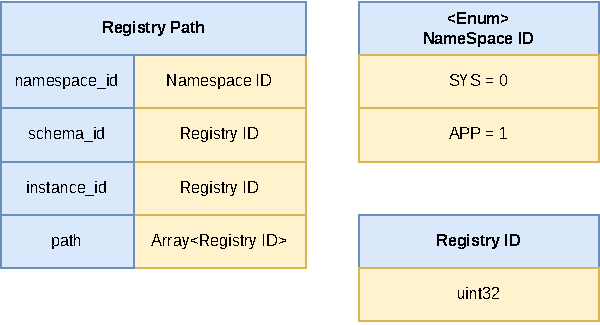
\includegraphics[width=0.8\textwidth]{data_structure_registry_path}
    \caption{\nameref{sec:design:riot_registry} \gls{ac:cp} implementation data structure.}
    \label{fig:riot_registry_path_structure}
\end{figure}

\section{\gls*{ac:api}}
\label{sec:implementation:riot_registry_api}

This section shows the implementation details of the in \autoref{sec:design:riot_registry:usage_flow} specified \gls{ac:api}.

\subsection{Basic \gls*{ac:api}}

\subsubsection{Get}

\autoref{fig:riot_registry_api_get} shows the implementation of how to get a configuration parameter's value as specified in \autoref{sec:design:riot_registry}.
It shows a function called ``get'' that takes a \gls{ac:cp} and a ``Registry Value'' pointer as an argument.
The ``Registry Value'' pointer is used to return the configuration parameter's value.

\begin{figure}[H]
    \centering
    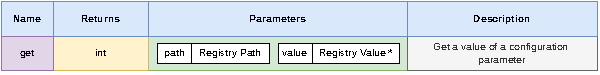
\includegraphics[width=\textwidth]{api_structure_get}
    \caption{\nameref{sec:design:riot_registry} \gls{ac:api}: get.}
    \label{fig:riot_registry_api_get}
\end{figure}

\autoref{lst:registry_get_function} shows the source code of this function.

\begin{lstlisting}[
    language=c,
    caption={Get configuration parameter values: C-function.},
    label={lst:registry_get_function},
]
int registry_get_value(
    const registry_path_t path,
    registry_value_t *value
);
\end{lstlisting}

\subsubsection{Set}

\autoref{fig:riot_registry_api_set} shows the implementation of how to set a configuration parameter's value to a new value as specified in \autoref{sec:design:riot_registry}.
It shows a function called ``set'' that takes a \gls{ac:cp} and a ``Registry Value'' as an argument.

\begin{figure}[H]
    \centering
    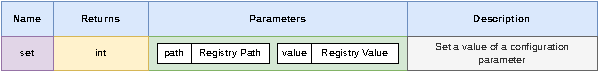
\includegraphics[width=\textwidth]{api_structure_set}
    \caption{\nameref{sec:design:riot_registry} \gls{ac:api}: set.}
    \label{fig:riot_registry_api_set}
\end{figure}

\autoref{lst:registry_set_function} shows the source code of this function.

\begin{lstlisting}[
    language=c,
    caption={Set new configuration parameter values: C-function.},
    label={lst:registry_set_function},
]
int registry_set_value(
    const registry_path_t path,
    const registry_value_t val
);
\end{lstlisting}

\subsubsection{Commit}

\autoref{fig:riot_registry_api_commit} shows the implementation of how to commit configuration parameters as specified in \autoref{sec:design:riot_registry}.
It shows a function called ``commit'' that takes a \gls{ac:cp} as an argument.

\begin{figure}[H]
    \centering
    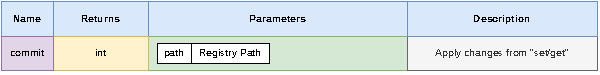
\includegraphics[width=\textwidth]{api_structure_commit}
    \caption{\nameref{sec:design:riot_registry} \gls{ac:api}: commit.}
    \label{fig:riot_registry_api_commit}
\end{figure}

\autoref{lst:registry_commit_function} shows the source code of this function.

\begin{lstlisting}[
    language=c,
    caption={Commit configuration parameters: C-function.},
    label={lst:registry_commit_function},
]
int registry_commit(const registry_path_t path);
\end{lstlisting}

\subsubsection{Export}

\autoref{fig:riot_registry_api_export} shows the implementation of how to export configuration parameters as specified in \autoref{sec:design:riot_registry}.
It shows a function called ``export'' that takes a \gls{ac:cp}, a callback function, a integer called ``recursion\_depth'' and a void pointer as for context data as an argument.
The ``recursion\_depth'' parameter of this function specifies how deep the export function is allowed to recursively search for configuration parameters and export them.
If the recursion\_depth is set to 0, then all configuration parameters, that are within the specified \gls{ac:cp} are exported.
If the recursion\_depth is set to 1, then only a configuration parameter gets exported, if it exactly matches the given \gls{ac:cp}.
If the recursion\_depth is set to a higher number than 1, the export function will export all configuration parameters, that are within the given \gls{ac:cp} and are not nested more steps deeper than the given \gls{ac:cp} goes plus the specified number.
The callback function takes a \gls{ac:cp}, a \gls{ac:cs}, a \gls{ac:si}, a ``Schema Item'' and a ``Registry Value'' and a void pointer for context data as its arguments.

\begin{figure}[H]
    \centering
    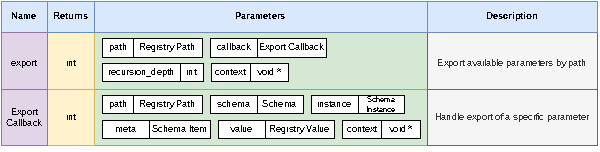
\includegraphics[width=\textwidth]{api_structure_export}
    \caption{\nameref{sec:design:riot_registry} \gls{ac:api}: export.}
    \label{fig:riot_registry_api_export}
\end{figure}

\autoref{lst:registry_export_function} shows the source code of this function.

\begin{lstlisting}[
    language=c,
    caption={Export configuration parameters: C-function.},
    label={lst:registry_export_function},
]
int registry_export(
    int (*export_func)(
        const registry_path_t path,
        const registry_schema_t *schema,
        const registry_instance_t *instance,
        const registry_schema_item_t *meta,
        const registry_value_t *value,
        const void *context
    ),
    const registry_path_t path,
    const int recursion_depth,
    const void *context,
);
\end{lstlisting}

\subsubsection{Load}

\autoref{fig:riot_registry_api_load} shows the implementation of how to load configuration parameter values from a non-volatile storage device as specified in \autoref{sec:design:riot_registry}.
It shows a function called ``load'' that takes a \gls{ac:cp} as an argument.

\begin{figure}[H]
    \centering
    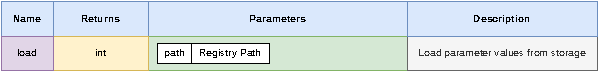
\includegraphics[width=\textwidth]{api_structure_load}
    \caption{\nameref{sec:design:riot_registry} \gls{ac:api}: load.}
    \label{fig:riot_registry_api_load}
\end{figure}

\autoref{lst:registry_load_function} shows the source code of this function.

\begin{lstlisting}[
    language=c,
    caption={Load configuration parameter values: C-function.},
    label={lst:registry_load_function},
]
int registry_load(const registry_path_t path);
\end{lstlisting}

\subsubsection{Save}

\autoref{fig:riot_registry_api_save} shows the implementation of how to save configuration parameter values to a non-volatile storage device as specified in \autoref{sec:design:riot_registry}.
It shows a function called ``save'' that takes a \gls{ac:cp} as an argument.

\begin{figure}[H]
    \centering
    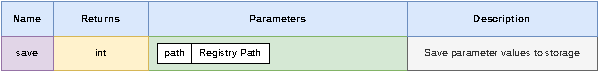
\includegraphics[width=\textwidth]{api_structure_save}
    \caption{\nameref{sec:design:riot_registry} \gls{ac:api}: save.}
    \label{fig:riot_registry_api_save}
\end{figure}

\autoref{lst:registry_save_function} shows the source code of this function.

\begin{lstlisting}[
    language=c,
    caption={Save configuration parameter values: C-function.},
    label={lst:registry_save_function},
]
int registry_save(const registry_path_t path);
\end{lstlisting}

\subsection{Schema Setup \gls*{ac:api}}

\autoref{fig:riot_registry_api_setup_schema} shows the implementation of how to register a \gls{ac:cs} or a \gls{ac:iot} in the \nameref{sec:design:riot_registry} as specified in \autoref{sec:design:riot_registry}.
It shows a function called ``register\_schema'' that takes a \gls{ac:cn} as an argument.
This function then adds the \gls{ac:cs} to a internal linked list.
\autoref{fig:riot_registry_api_setup_schema} also shows a function called ``register\_schema\_instance'', which takes a \gls{ac:cn}, a \gls{ac:cs} ID and a pointer to a \gls{ac:si} as its argument.
Internally the \nameref{sec:design:riot_registry} then adds the \gls{ac:si} to the linked list of \glspl{ac:si}, stored in the \gls{ac:cs} that matches the given \gls{ac:cs} ID.

\begin{figure}[H]
    \centering
    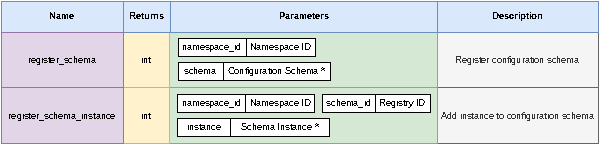
\includegraphics[width=\textwidth]{api_structure_setup_schema}
    \caption{\nameref{sec:design:riot_registry} \gls{ac:api}: setup \gls{ac:cs}.}
    \label{fig:riot_registry_api_setup_schema}
\end{figure}

\autoref{lst:registry_schema_setup_api} shows the source code of these functions.

\begin{lstlisting}[
    language=c,
    caption={Schema Setup \gls{ac:api}.},
    label={lst:registry_schema_setup_api},
]
void registry_schemas_init(void);

int registry_register_schema(
    const registry_namespace_id_t namespace_id,
    const registry_schema_t *schema
);

int registry_register_schema_instance(
    const registry_namespace_id_t namespace_id,
    const registry_id_t schema_id,
    const registry_instance_t *instance
);
\end{lstlisting}

\subsection{\acrlong*{ac:sf} Setup \gls*{ac:api}}

\autoref{fig:riot_registry_api_setup_storage_facility} shows the implementation of how to register a \gls{ac:sf} in the \nameref{sec:design:riot_registry} as specified in \autoref{sec:design:riot_registry}.
It shows a function called ``register\_storage\_facility\_src'' that takes a pointer to a \gls{ac:sf} Instance as an argument.
This function then adds the \gls{ac:sf} Instance to a internal linked list of \gls{ac:sf} sources.
\autoref{fig:riot_registry_api_setup_storage_facility} also shows a function called ``register\_storage\_facility\_dst'' that takes a pointer to a \gls{ac:sf} Instance as an argument.
This function then sets the \gls{ac:sf} Instance as the internal \gls{ac:sf}.
This \gls{ac:sf} is not added to a internal linked list, because there can only be one \gls{ac:sf} to write to.

\begin{figure}[H]
    \centering
    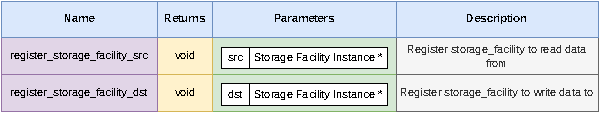
\includegraphics[width=\textwidth]{api_structure_setup_storage_facility}
    \caption{\nameref{sec:design:riot_registry} \gls{ac:api}: Setup \gls{ac:sf}.}
    \label{fig:riot_registry_api_setup_storage_facility}
\end{figure}

\autoref{lst:registry_storage_facility_setup_api} shows the source code of these functions.

\begin{lstlisting}[
    language=c,
    caption={\acrlong{ac:sf} Setup \gls{ac:api}.},
    label={lst:registry_storage_facility_setup_api},
]
void registry_register_storage_facility_src(
    const registry_storage_facility_instance_t *src
);

void registry_register_storage_facility_dst(
    const registry_storage_facility_instance_t *dst
);
\end{lstlisting}


\chapter{Testing of the Implementation's Correctness}
\label{chapter:testing}

The ``registry\_tests'' module provides unit tests that can be run by including the ``registry\_tests.h'' header file and calling the ``registry\_tests\_api\_run'' function.

\section{Test Setup}

To be able to test if all by the \nameref{sec:design:riot_registry} supported data types are supported, the ``registry\_tests'' module uses the ``registry\_schema\_full\_example'' of the ``registry\_schemas'' module.
This \gls{ac:cs} contains fields for every supported data type of the \nameref{sec:design:riot_registry} (see \autoref{sec:requirements:typed_configuration_parameters} and \autoref{fig:riot_registry_configuration_parameter_type_enum}).
Additionally the module creates and registers a custom \gls{ac:cs} called ``registry\_schema\_groups\_test'', which consists of 4 \glspl{ac:cg}, that are children of each other, creating a maximum \gls{ac:cp} of up to 5 segments excluding the \gls{ac:cn}, \gls{ac:cs} and \gls{ac:si}.
This is necessary to test if the \glspl{ac:cg} are implemented correctly.

\section{Testing the ``registry\_get'' and ``registry\_set'' Functions}
\label{sec:testing:get_and_set}

To test the correctness of the ``registry\_get'' and ``registry\_set'' functions of the \nameref{sec:design:riot_registry}, first we call the ``registry\_set'' function for all fields of the ``registry\_schema\_full\_example'' \gls{ac:cs} and also for all fields of the ``registry\_schema\_groups\_test'' \gls{ac:cs} to test every data type that is supported by the \nameref{sec:design:riot_registry} and also if \glspl{ac:cg} work.
Then we call the ``registry\_get'' function for all previously set parameters and compare the returning values to the original values.
If these values match, the test is successful.
This testing sequence is executed for the minimum and maximum value for each configuration parameter.

\section{Testing the ``registry\_commit'' Function}

To test the correctness of the ``registry\_commit'' function of the \nameref{sec:design:riot_registry}, first we create a global bool and initialize it to ``false''. Then we call the ``registry\_commit'' function providing a \gls{ac:cp} as an argument that points to a configuration parameter of a \gls{ac:si}, which in its callback function checks, if the provided values are matching to what is expected. It then changes the value of the global bool to ``true'' if the values are correct and to ``false'' if they are not.
If the value is set to ``true'', the test is successful.

Ideally this test is not only implemented for calling a concrete configuration parameter of a \gls{ac:si}, but also for calling incomplete \glspl{ac:cp}, such as a \gls{ac:cp} that only points to the \gls{ac:cs} or one that only points to the \gls{ac:si}.
In both cases the configuration parameter must be committed because its parent got committed.
These tests are not yet implemented.

\section{Testing the ``registry\_export'' Function}

To test the correctness of the ``registry\_export'' function of the \nameref{sec:design:riot_registry}, first we create a global bool and initialize it to ``false''. Then we call the ``registry\_export'' function providing a \gls{ac:cp} that points to a configuration parameter and a custom callback function as its arguments. When the callback function gets called, it checks if the provided values are matching to what is expected. It then changes the value of the global bool to ``true'' if the values are correct and to ``false'' if they are not.
If the value is set to ``true'', the test is successful.

Ideally this test is not only implemented for calling a concrete configuration parameter of a \gls{ac:si}, but also for calling incomplete \glspl{ac:cp}, such as a \gls{ac:cp} that only points to the \gls{ac:cs} or one that only points to the \gls{ac:si}.
In these cases it depends on the ``recursion'' argument, how deep the ``registry\_export'' function searches inside the \gls{ac:cs} for configuration parameters to export.
These tests are not yet implemented.

\section{Testing the ``registry\_save'' and ``registry\_load'' Function}

To test the ``registry\_save'' and ``registry\_load'' functions, every test that is done in \ref{sec:testing:get_and_set} gets executed again, but this time after each sequence we call the ``registry\_save'' function to write the values to the storage.
Then all previously set configuration parameters get changed to a different value using the ``registry\_set'' function.
And finally we call the ``registry\_load'' function to read the values written to storage and loading them into the \nameref{sec:design:riot_registry} again.
If these values now match with the values that were initially set by the ``registry\_set'' function,
then the test is successful.
\chapter{Evaluation of the implementation's overhead}
\label{chapter:evaluation}

\section{RAM}
\label{sec:evaluation:ram_overhead}

\subsection{Heap}

The \nameref{sec:design:riot_registry} does not do any dynamic heap allocations, so evaluating the heap overhead is not necessary.

\subsection{Stack}

In this section the stack consumption of the \nameref{sec:design:riot_registry} \gls{ac:api} is measured and discussed.
More specifically the functions ``registry\_get\_value'', registry\_set\_value, ``registry\_commit'', ``registry\_export'', ``registry\_save'' and ``registry\_load'' are measured.

\subsubsection{Method}

To measure the stack usage of a function in \gls{gl:riot_os} is possible, because the stack implementation internally marks parts of the stack that have been ``touched''.
This way the highest ever used stack count can be printed out, but this also has the downside that before starting the measurement, the currently highest measured stack count must be equal to the current stack count.
This can be achieved by creating a new thread, which start stack count is equal to the highest stack count until that moment.

This leads to the following stack consumption measurement strategy:
\begin{enumerate}
    \item Create a new thread.
    \item Get the current stack count (highest).
    \item Save the current stack count to a variable.
    \item Call the function which stack consumption needs to be measured.
    \item Get the highest stack count.
    \item Subtract the old stack count from the new stack count.
    \item Print out the result to the terminal.
\end{enumerate}

\subsubsection{Measurements}

\autoref{table:stack_overhead} and \autoref{fig:evaluation:stack_overhead_chart} show the result of this measurement in bytes.
The first row of \autoref{table:stack_overhead} tells the length of the \gls{ac:cp}, all following rows show the stack consumption of each function per \gls{ac:cp} length.
The result shows that almost all functions don't increase their overall stack consumption at all if the \gls{ac:cp} length changes.
One exception is ``registry\_export'', which has a increase of 16 bytes (+1.5\%) from a \gls{ac:cp} with the length of 1 to a \gls{ac:cp} with the length of 2 and it also has another increase of 16 bytes from a \gls{ac:cp} with the length of 4 to a \gls{ac:cp} with the length of 5.
The other exception is the function ``registry\_save'', which oscillates between a stack consumption of up to 3,900 and down to 3,340.

\begin{table}[H]
    \begin{tabular}{ | l | r | r | r | r | r | }
        \hline
        Function \textbackslash{ \gls{ac:cp} length} & 1     & 2     & 3     & 4     & 5
        \\ \hline
        registry\_get\_value                         & 276   & 276   & 276   & 276   & 276   \\ \hline
        registry\_set\_value                         & 308   & 308   & 308   & 308   & 308   \\ \hline
        registry\_commit                             & 464   & 464   & 464   & 464   & 464   \\ \hline
        registry\_export                             & 1,092 & 1,108 & 1,108 & 1,108 & 1,124 \\ \hline
        registry\_save                               & 3,884 & 3,340 & 3,900 & 3,340 & 3,356 \\ \hline
        registry\_load                               & 2,636 & 2,636 & 2,636 & 2,636 & 2,636 \\ \hline
    \end{tabular}
    \caption{Stack consumption of \nameref{sec:design:riot_registry} \gls{ac:api} functions in bytes.}
    \label{table:stack_overhead}
\end{table}

\autoref{fig:evaluation:stack_overhead_chart} shows the stack consumption of each main \nameref{sec:design:riot_registry} function on the y axis in bytes.
The x axis shows the length of the \gls{ac:cp} that was passed to each function.

\begin{figure}[H]
    \centering
    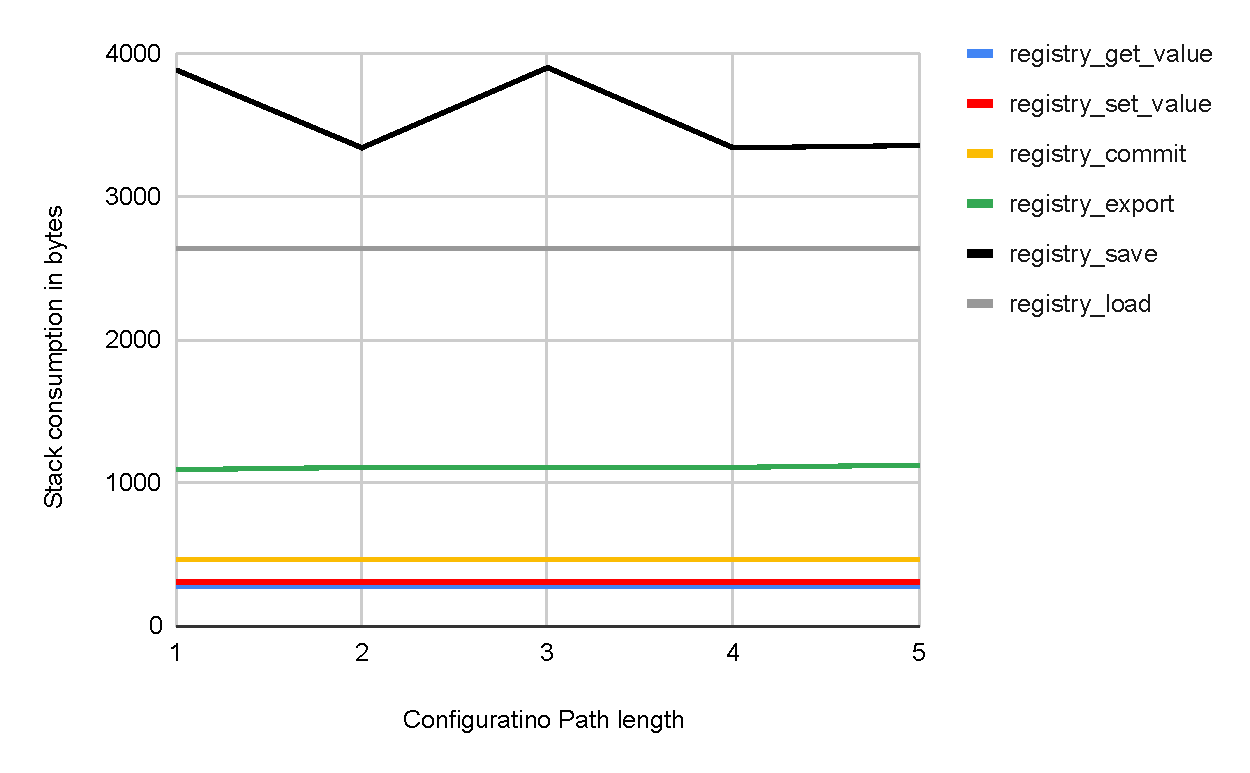
\includegraphics[width=\textwidth]{evaluation_stack_consumption_chart}
    \caption{\nameref{sec:design:riot_registry} stack consumption in bytes per \gls{ac:api} function on the \gls{ac:cp} lengths 0 - 5.}
    \label{fig:evaluation:stack_overhead_chart}
\end{figure}

\subsubsection{Discussion}

Overall the results of these measurements are not unexpected and possible to explain.
The ``set'' and ``get'' function are implemented without recursion and should not consume more stack only because they need to go deeper into the \gls{ac:cs} structure.
The ``commit'' function has a similar implementation to the ``get'' and ``set'' functions, but still consumes more stack because its slightly more complex implementation is currently distributed among multiple functions that call each other and it also needs to call the callback function of the \gls{ac:si} to inform the driver / module about the to be applied changes (see \autoref{fig:behavioral_flow_of_the_commit_api} and \autoref{fig:behavioral_flow_of_the_set_api} for comparison).
The ``export'' function is similar implemented to the ``commit'' function (see \autoref{fig:behavioral_flow_of_the_export_api}) and has its logic distributed among multiple functions, that call each other.
The major difference, that also causes the much higher stack usage is that each of these functions take up to 7 times more arguments.

The stack consumption of the ``registry\_save'' and ``registry\_load'' functions however  are more difficult to discuss.
In this example both use a \gls{ac:sf} that internally uses the \gls{gl:riot_os} \gls{ac:vfs} layer, which abstracts over filesystems such as FatFs or littlefs.
In this case the littlefs abstraction is used.
What happens with littlefs internally is unknown, but the measurements behave reasonable in contrast to how the \gls{ac:vfs} \gls{ac:sf} is implemented.
Both functions do not use recursive function calls and only rely on while loops that reuse data structures.
As a consequence also these two function don not consume more stack in relation to the \gls{ac:cp} length.
But this conclusion is only valid for the \gls{ac:vfs} \gls{ac:sf}.
Other implementations may show different results.

In general the implementation of all the analyzed functions can be improved.
Especially the distribution into multiple functions that call each other by passing on a lot of arguments is not ideal.
It makes the source code less difficult to maintain, but has the consequence of consuming unnecessarily much stack.
It should theoretically be possible to make the functions ``get'', ``set'', ``commit'' and ``export'' consume almost the same amount of stack with a more better implementation.
Of course there would still be some differences caused by the different requirements of these functions. Such things as the callback of the ``commit'' function.

\section{ROM}
\label{sec:evaluation:rom_overhead}

\gls{gl:riot_os} has a tool called ``Cosy''.
It can be used as a build target and analyzes the last build binary size in different categories.
To compare the ROM size of a \gls{gl:riot_os} application with and without the \nameref{sec:design:riot_registry}, the application is analyzed by the given tool.

\subsection{Full Binary Size Comparison}

\subsubsection{Method}

First, the ROM size of a sample \gls{gl:riot_os} application is measured with all \nameref{sec:design:riot_registry} modules disabled in the makefile.
Then the \nameref{sec:design:riot_registry} modules get enabled one by one and new measurements are taken. At the end the ROM size of all modules together is measured as well.
Subtracting the initial ROM size with all \nameref{sec:design:riot_registry} modules disabled from the measurements that enable some additional \nameref{sec:design:riot_registry} modules, allows to see the actual ROM size cost of using the \nameref{sec:design:riot_registry} modules.

\subsubsection{Measurements}

The measured size in bytes of the sample application without any \gls{gl:riot_os} modules enabled can be seen in \autoref{table:rom_size_without_any_riot_registry_modules_enabled}.
The measurements with each module separately enabled and also all at once can be seen in \autoref{table:rom_overhead_with_dependencies}, which shows the name of the enabled modules in column one, the total measured ROM size in bytes in column two, the difference between with and without the module can be found in column three in bytes and in column 4 in percentage relative to the ROM size without any \nameref{sec:design:riot_registry} modules enabled.

\begin{table}[H]
    \begin{tabular}{ | l | r | }
        \hline
        Enabled \nameref{sec:design:riot_registry} module(s) & Size in bytes
        \\ \hline
        -                                                    & 1,386,602
        \\ \hline
    \end{tabular}
    \caption{ROM size without any \nameref{sec:design:riot_registry} modules enabled.}
    \label{table:rom_size_without_any_riot_registry_modules_enabled}
\end{table}

\begin{table}[H]
    \begin{tabular}{ | l | r | r | r | }
        \hline
        \begin{tabular}[x]{@{}c@{}}Enabled \gls{gl:riot_os}                             \\ Registry module(s)\end{tabular}     & Size in bytes & Difference in bytes & Difference in \%
        \\ \hline
        registry                      & 1,437,782     & +51,180             & +3.7             \\ \hline
        registry\_schemas             & 1,416,356     & +29,754             & +2.1             \\ \hline
        registry\_storage\_facilities & 1,419,947     & +33,345             & +2.4             \\ \hline
        registry\_cli                 & 1,407,312     & +20,710             & +1.5             \\ \hline
        All registry\_* modules       & 1,503,139     & +116,537            & +8.4             \\ \hline
    \end{tabular}
    \caption{ROM size of \nameref{sec:design:riot_registry} modules and their overhead in bytes and percentage.}
    \label{table:rom_overhead_with_dependencies}
\end{table}

\subsubsection{Discussion}

It should be noted that if the ROM size differences of each \nameref{sec:design:riot_registry} module get accumulated, the result (134,989) is 18,452 bytes larger then if all \nameref{sec:design:riot_registry} modules are enabled together. This is caused by shared dependencies that get optimized by the compiler.

Besides the \nameref{sec:design:riot_registry} modules listed in \autoref{table:rom_overhead_with_dependencies}, there is also the ``registry\_tests'' module.
This module only contains tests and is not needed when using the \nameref{sec:design:riot_registry} inside an application.
That is why it is not part of \autoref{table:rom_overhead_with_dependencies}, which means it is also not part of the ``All registry\_* modules'' enabled row.

\subsection{Compiled Object Sizes}

\subsubsection{Method}

The "Cosy" tool also allows to show the exact size of compiled object files.
This allows to get a more precise view of how much ROM is exactly used per module implementation.

\subsubsection{Measurements}

To be able directly compare with the previous measurements listed in \autoref{table:rom_overhead_with_dependencies}, in \autoref{table:compiled_object_file_size_of_riot_registry_modules} the object file sizes are not provided alone, but also accumulated per \gls{gl:riot_os} module.
By comparing the sizes of column 2 in \autoref{table:compiled_object_file_size_of_riot_registry_modules} to the calculated differences in column 3 of \autoref{table:rom_overhead_with_dependencies}, it can be said, that each of the corresponding values have around the same size.
In most cases the object files based module size is between 3 to 4.5 kilobytes smaller, except in case of the ``registry'' module, which is around 4.5 kilobytes larger then the measurement of \autoref{table:rom_overhead_with_dependencies}.

\begin{table}[H]
    \begin{tabular}{|l|r|l|r|}
        \hline
        Module                                     & \begin{tabular}[x]{@{}c@{}}Module size \\ in bytes\end{tabular} & Object file                         & \begin{tabular}[x]{@{}c@{}}Object file size \\ in bytes\end{tabular} \\

        % registry
        \hline
        \multirow{2}{*}{registry}                  & \multirow{2}{*}{55,678}   & registry.o                          &
        39,447                                                                                                                                   \\
        \cline{3-4}
                                                   &                           & registry\_conversion.o              & 16,231                    \\
        % registry_schemas
        \hline
        \multirow{3}{*}{registry\_schemas}         & \multirow{3}{*}{25,219}   & registry\_schemas\_init.o           &
        5,726                                                                                                                                    \\
        \cline{3-4}
                                                   &                           & registry\_schema\_rgb\_led.o        & 8,834                     \\
        \cline{3-4}
                                                   &                           & registry\_schema\_full\_example.o   & 10,659                    \\

        % registry_storage_facilities
        \hline
        \multirow{2}{*}{\begin{tabular}[l]{@{}l@{}}registry\_\\storage\_facilities\end{tabular}} & \multirow{2}{*}{30,335}   & registry\_storage\_facility\_vfs.o  &
        21,189                                                                                                                                   \\
        \cline{3-4}
                                                   &                           & registry\_storage\_facility\_heap.o & 9,146                     \\

        % registry_cli
        \hline
        registry\_cli                              & 17,824                    & registry\_cli.o                     & 17,824                    \\

        % registry_tests
        \hline
        \multirow{2}{*}{registry\_tests}           & \multirow{2}{*}{53,128}   & registry\_tests\_stack.o            &
        32,597                                                                                                                                   \\
        \cline{3-4}
                                                   &                           & registry\_tests\_api.o              & 20,531                    \\
        \hline
    \end{tabular}
    \caption{Compiled object file size of \nameref{sec:design:riot_registry} modules.}
    \label{table:compiled_object_file_size_of_riot_registry_modules}
\end{table}

\autoref{fig:evaluation:rom_usage_per_module} shows the same results as \autoref{table:compiled_object_file_size_of_riot_registry_modules}, but as a donut diagram to better understand the relation between the measured objects.
The inner circle represents the \nameref{sec:design:riot_registry} modules and the outer circle represents the corresponding object files that were compiled from the c-files implementing these modules.

\begin{figure}[H]
    \centering
    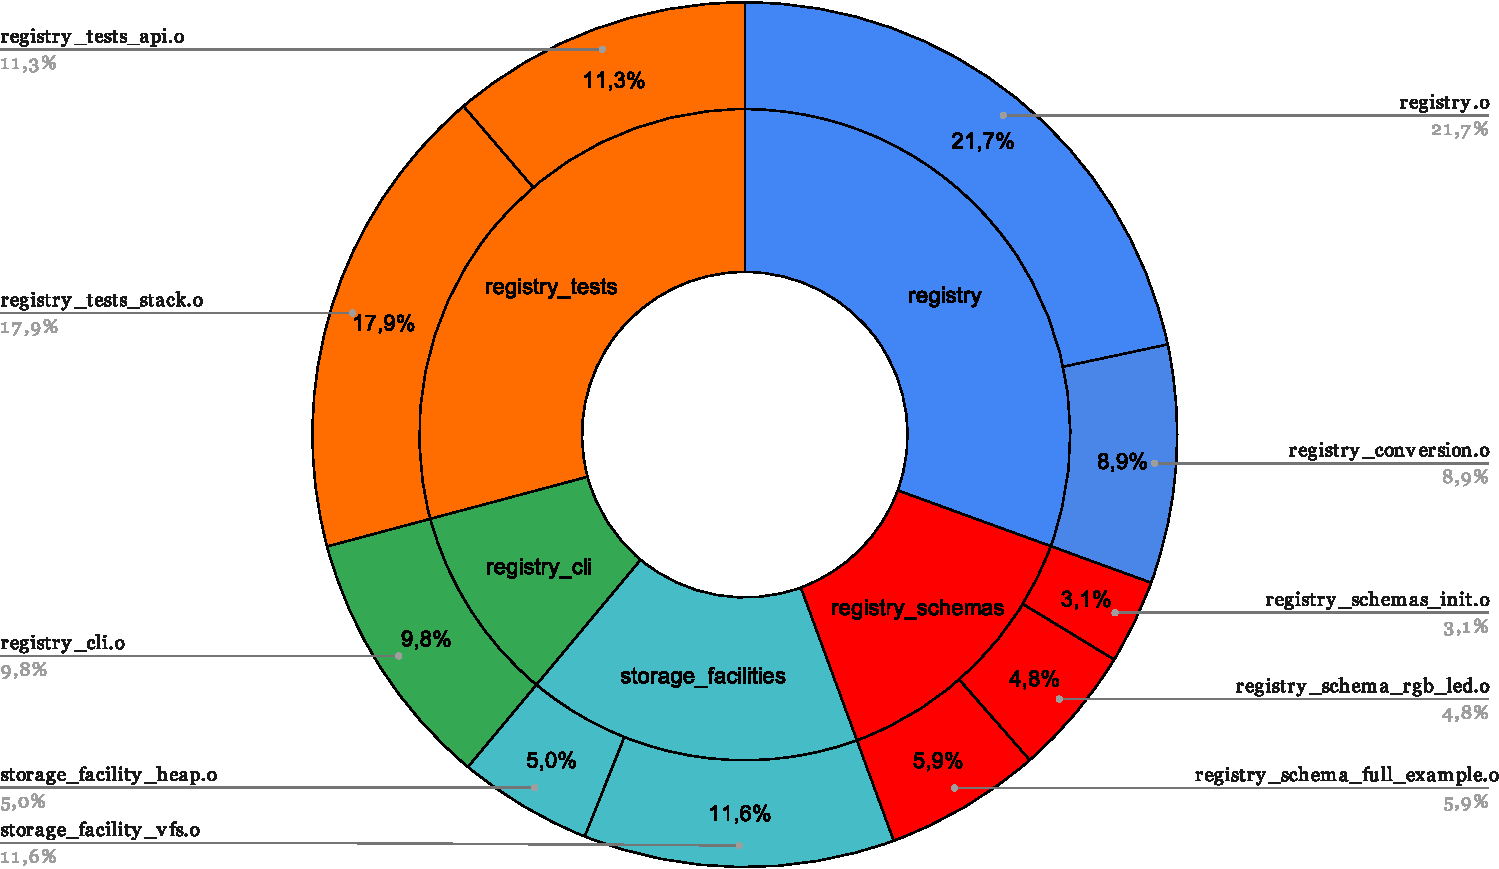
\includegraphics[width=\textwidth]{evaluation_rom_pie_chart}
    \caption{\nameref{sec:design:riot_registry} ROM usage per module (inner circle) and per object file (outer circle).}
    \label{fig:evaluation:rom_usage_per_module}
\end{figure}

\subsubsection{Discussion}

The more fine-grained measurements are helpful because the ``registry\_schemas'' and ``registry\_storage\_facilites'' modules allow to enable and disable each \gls{ac:cs} and \gls{ac:sf} implementation separately.
This way a lot of ROM overhead can be avoided by only enabling what is needed and these measurements show about how much can be saved.

It should also be noted that the ``registry\_tests'' module is usually not enabled when using the \nameref{sec:design:riot_registry}.
\chapter{Future Work}
\label{chapter:future_work}

\section{Full Test Coverage}

As mentioned in \ref{chapter:testing}, the currently implemented tests don't have the highest test coverage yet.
In the future the unit tests of the \nameref{sec:design:riot_registry} should be extended to find and prevent more implementation mistakes.

\section{Exposing Configuration Parameters Beyond Abstraction}

Investigate how to expose custom config data beyond abstraction:
Some sensors have very specific configuration parameters that can not all be sufficiently abstracted through one large interface.
Possible solutions:

\begin{itemize}
    \item Implement custom \gls{ac:cs} for these sensors.

    \item Expose those parameters through a field in every \gls{ac:cs} that can hold additional parameters and is not type-safe.
          Set, Get handlers and persistence must be implemented by the driver itself and not the \gls{ac:cs} in this case.
\end{itemize}

\section{Extend Configuration Parameter Value Constraints}

Investigate how to expose further value constraints of configuration parameters.
Configuration parameters, in the case of numbers, usually for example don't expect the full range that the size of a primitive c-type (8, 16, 32 or 64-bit) allows.
In some cases maybe even only a certain set of specifically selected values is a correct configuration value.
There should be a way to specify how to expose those constraints through the Registry \gls{ac:api} through additional metadata fields.
Possible use-cases:

\begin{itemize}
    \item Constrain the minimum and maximum value of a numeric configuration parameter.

    \item Constrain the minimum and maximum length of a (string) configuration parameter.

    \item Specifies a set of values that are allowed to be set.
          This gives the possibility to implicitly define an ``enum'' like configuration parameter.
\end{itemize}

\section{External \gls*{gl:configuration_manager} Implementation}

This thesis only specifies the architectural design of how \gls{ac:coap}, \gls{gl:mqtt} and \gls{gl:lwm2m} can be used to implement external \glspl{gl:configuration_manager} for the \gls{gl:riot_os} and only implements a \gls{ac:cli} for external configuration management (see \autoref{sec:design:integrating_external_configuration_managers:simple_configuration_managers:cli}).
Those integrations still need to be implemented.

\begin{itemize}
    \item \gls{ac:coap} based \gls{ac:api} (uses registry structure).

    \item \gls{gl:mqtt} based \gls{ac:api} (uses registry structure).

    \item \gls{gl:lwm2m} mapping (\nameref{sec:design:riot_registry} => \gls{gl:lwm2m} Object Models).
\end{itemize}

\section{Specification of Sys \acrlongpl*{ac:cs}}
\label{sec:future_work:specification_of_schemas_for_common_use_cases}

As of now the \nameref{sec:design:riot_registry} only comes with two simple example \glspl{ac:cs} in its ``sys'' \gls{ac:cn}, one being an LED-RGB \gls{ac:cs} to control the color of an rgb LED, and the other being a \gls{ac:cs} with the name ``full\_example'' that contains all supported parameter types for testing.
To give modules/drivers the ability to implement \glspl{ac:cs}, first those \glspl{ac:cs} must be defined.
This is no simple task as each \gls{ac:cs} must be specified in a way that is compatible to as many as possible drivers of the same kind.

\section{Integration of the \nameref*{sec:design:riot_registry} into \gls*{gl:riot_os} Modules and Drivers.}

After a \gls{ac:cs} is specified as explained in \autoref{sec:future_work:specification_of_schemas_for_common_use_cases}, it has to be implemented by the compatible modules/drivers that need runtime configuration.

\chapter{Conclusion}
\label{chapter:conclusion}

Our main goal of this thesis to specify a runtime configuration registry for \gls{gl:riot_os} has been achieved (see \autoref{chapter:design}).
The implementation (see \autoref{chapter:implementation}) has also been successful and fulfills all the requirements specified in \autoref{chapter:requirements}.

Looking back and around to see what has already been done prior to this thesis in \autoref{chapter:related_work} has been very helpful for us to get an overview of in what ways \glspl{ac:rcs} have been designed so far and for which use-cases.
Thinking about the use-cases of already existing solutions helped in specifying use-cases and requirements that are relevant to fulfill, for the \gls{gl:riot_os} implementation even if the related work was not exactly what is needed for a \gls{gl:riot_os} \gls{ac:rcs}.
This in turn helped us to assess how much the in \autoref{chapter:related_work} assessed already existing implementations are capable of fulfilling these \gls{gl:riot_os}-specific requirements (see \autoref{chapter:requirements} and \autoref{chapter:related_work} \autoref{sec:related_work:assessment_of_implementation_work_on_thesis_requirements}).
We learned that none of the assessed already existing implementations fulfill all the requirements of \autoref{chapter:requirements}, but we were able to base the new \nameref{sec:design:riot_registry} on the existing \gls{ac:mynewt_config} implementation for \gls{gl:riot_os}, which helped speed up the development process by a lot.
Our final design (see \autoref{chapter:design}) turned out much different to from where it started (\gls{ac:mynewt_config}), but the main \gls{ac:api} functions are still roughly the same.

Writing unit tests (see \autoref{chapter:testing}) helped not only finding a lot of bugs in the \nameref{sec:design:riot_registry} implementation, but also helped in creating new ones while further iterating on the \nameref{sec:design:riot_registry}'s implementation.
Which is why, it is of high importance to further increase the testing coverage as mentioned in \autoref{chapter:future_work}.

\autoref{chapter:evaluation} showed us that our implementation's overhead is acceptable for devices with enough memory (stack overhead up to > 4 kilobyte) and it does not perform any dynamic heap allocations, but there are still many ways to further reduce its stack overhead.

For the future it will be very interesting to see how good the new \nameref{sec:design:riot_registry} can specify \glspl{ac:cs} that abstract common configuration parameters shared by the many \gls{gl:riot_os} modules and drivers (see \autoref{sec:future_work:specification_of_schemas_for_common_use_cases}).

\nocite{never_gonna_give_you_up}

% Add additional chapters here

%\bibliographystyle{plain}
\bibliographystyle{IEEEtran}
\bibliography{
  literature/general,
  literature/bib/iot,
  literature/bib/ids,
  literature/bib/rfcs,
  literature/bib/own,
  literature/bib/programming
}

% Appendix
% \appendix
% \chapter{asdf}


\IGlossary

\Istatement

\end{document}
